\documentclass[report.tex]{subfiles}
\graphicspath{ \subfix{./images/} \subfix{./graphs/} }
\begin{document}
\chapter{Evaluation}

\section{Alpha testing}

\subsection{Unit test and code coverage}

Throughout the development process, I have written a total of 55 test cases. Running all of them takes around 20 seconds and they test all the code in the core library, making it bug-free when integrating with the user interface.

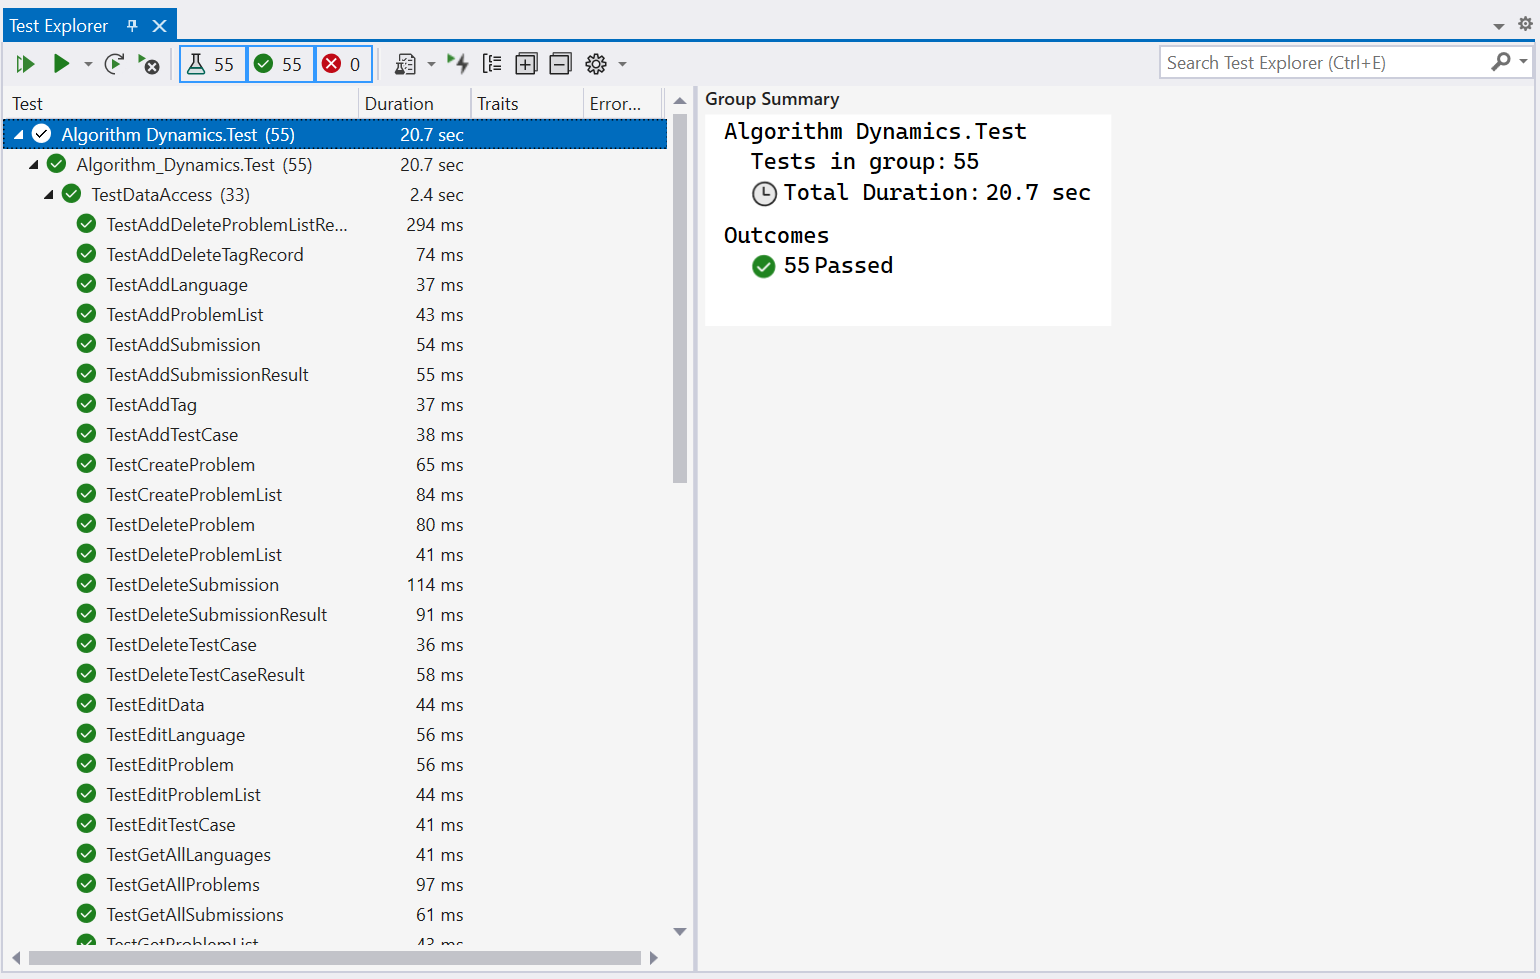
\includegraphics[width=\textwidth, height=\textheight, keepaspectratio]{UnitTestUI}

The overall test coverage is 88.4\%. The coverage is a measurement of how many lines of code are executed during the unit tests. 88.4\% is a very high percentage, some of the untested code are helper functions and dummy properties. The coverage is not a measure of the quality of the code, but rather the quality of the tests and I am confident that with all those unit tests, the core library is bug-free.

\subsection{Code Metrics}

I ran the code analysis on the entire codebase and it gives me a maintainability index. It calculates an index value between 0 and 100 that represents the relative ease of maintaining the code. A high value means better maintainability. Colour-coded ratings can be used to quickly identify trouble spots in your code. A green rating is between 20 and 100 and indicates that the code has good maintainability.\cite{microsoft:docs:code-metrics-maintainability-index-range-and-meaning}

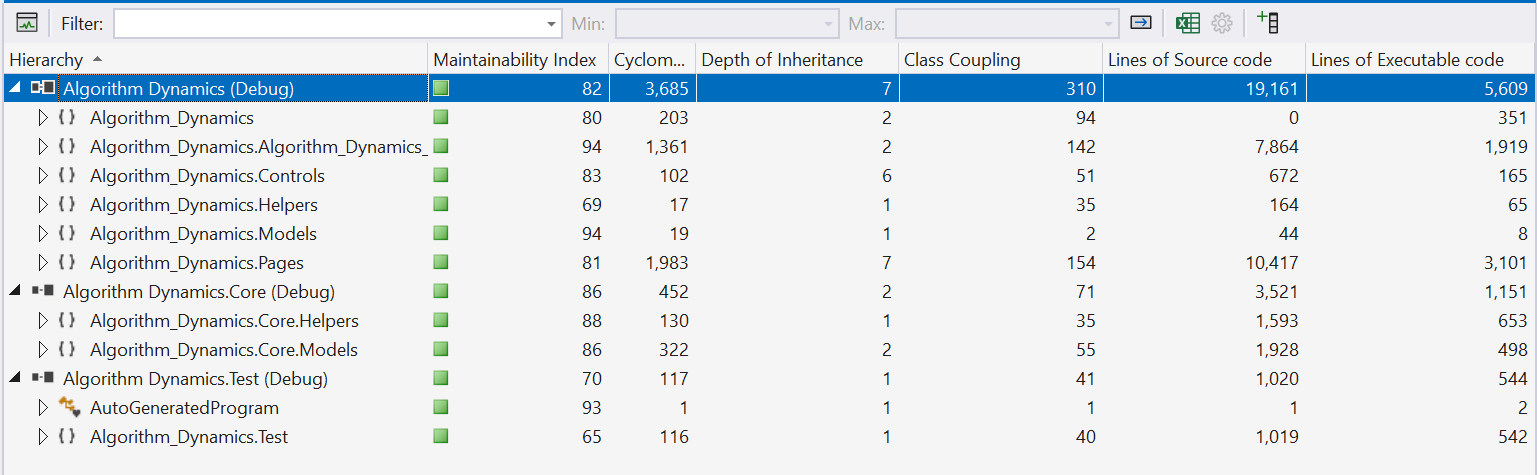
\includegraphics[width=\textwidth, height=\textheight, keepaspectratio]{CodeAnalysis}

\subsection{Usability testing}

\subsubsection{NavigationView}

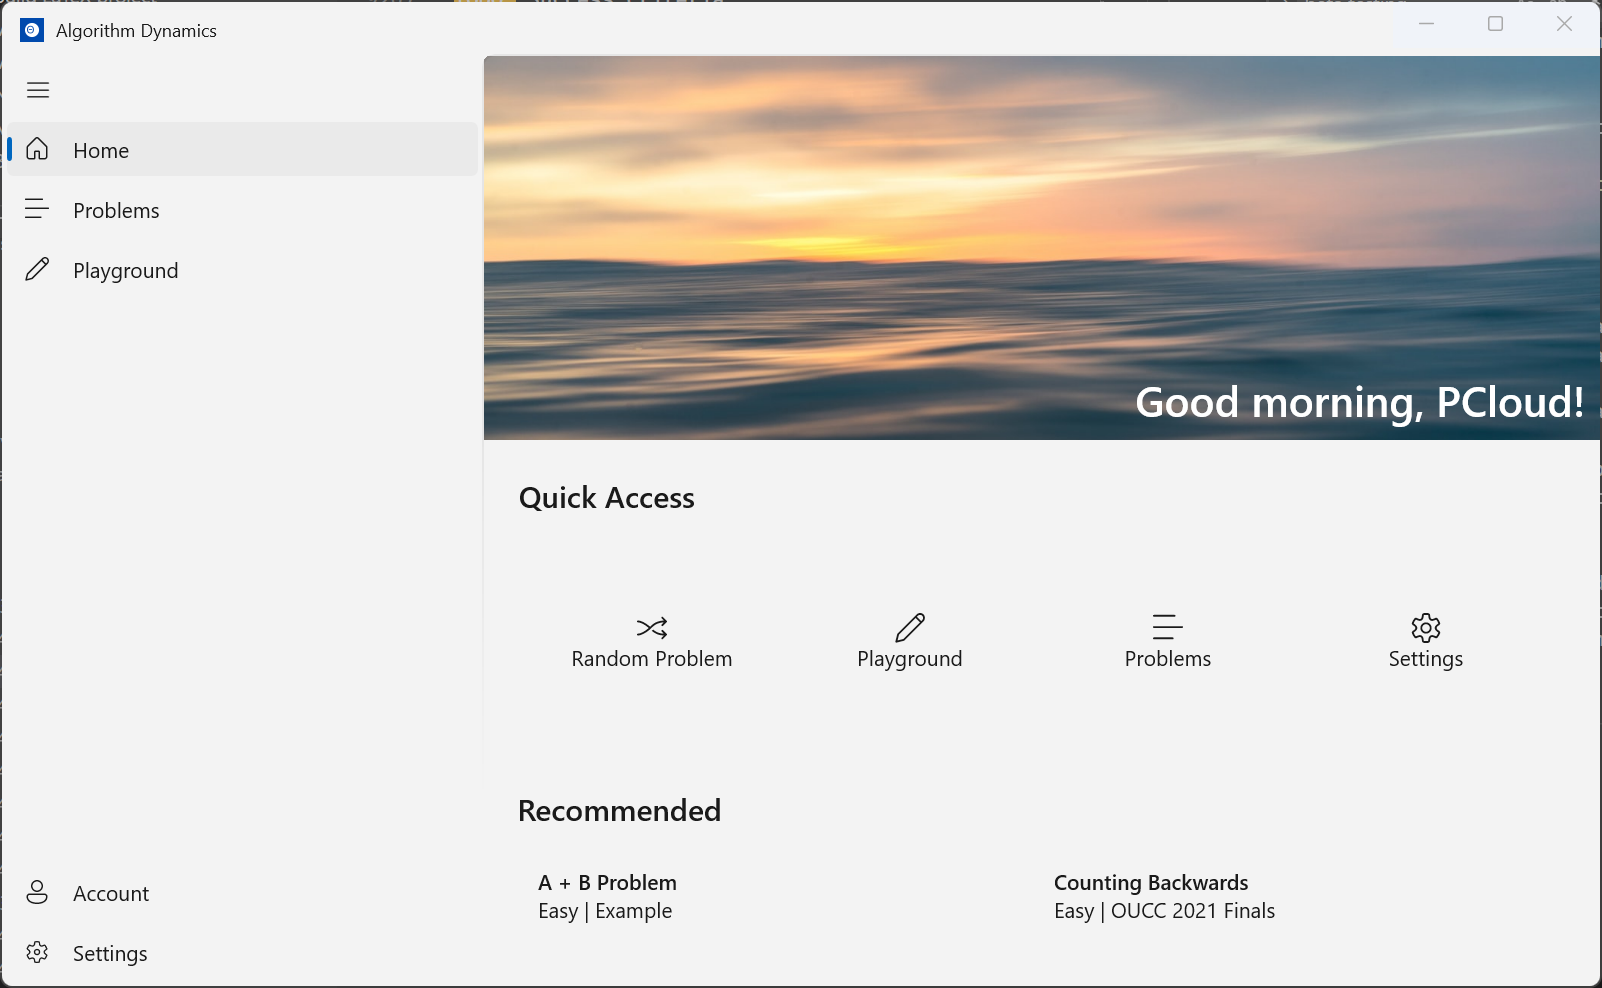
\includegraphics[width=\textwidth, height=\textheight, keepaspectratio]{HomePage-Final}

\begin{tabulary}{\linewidth}{|L|l|}
    \hline
    Test & Result \\
    \hline
    Does it load & Pass \\
    \hline
    Does the button work & Pass \\
    \hline
    Does it response to different screen size & Pass \\
    \hline
\end{tabulary}

\subsubsection{HomePage}

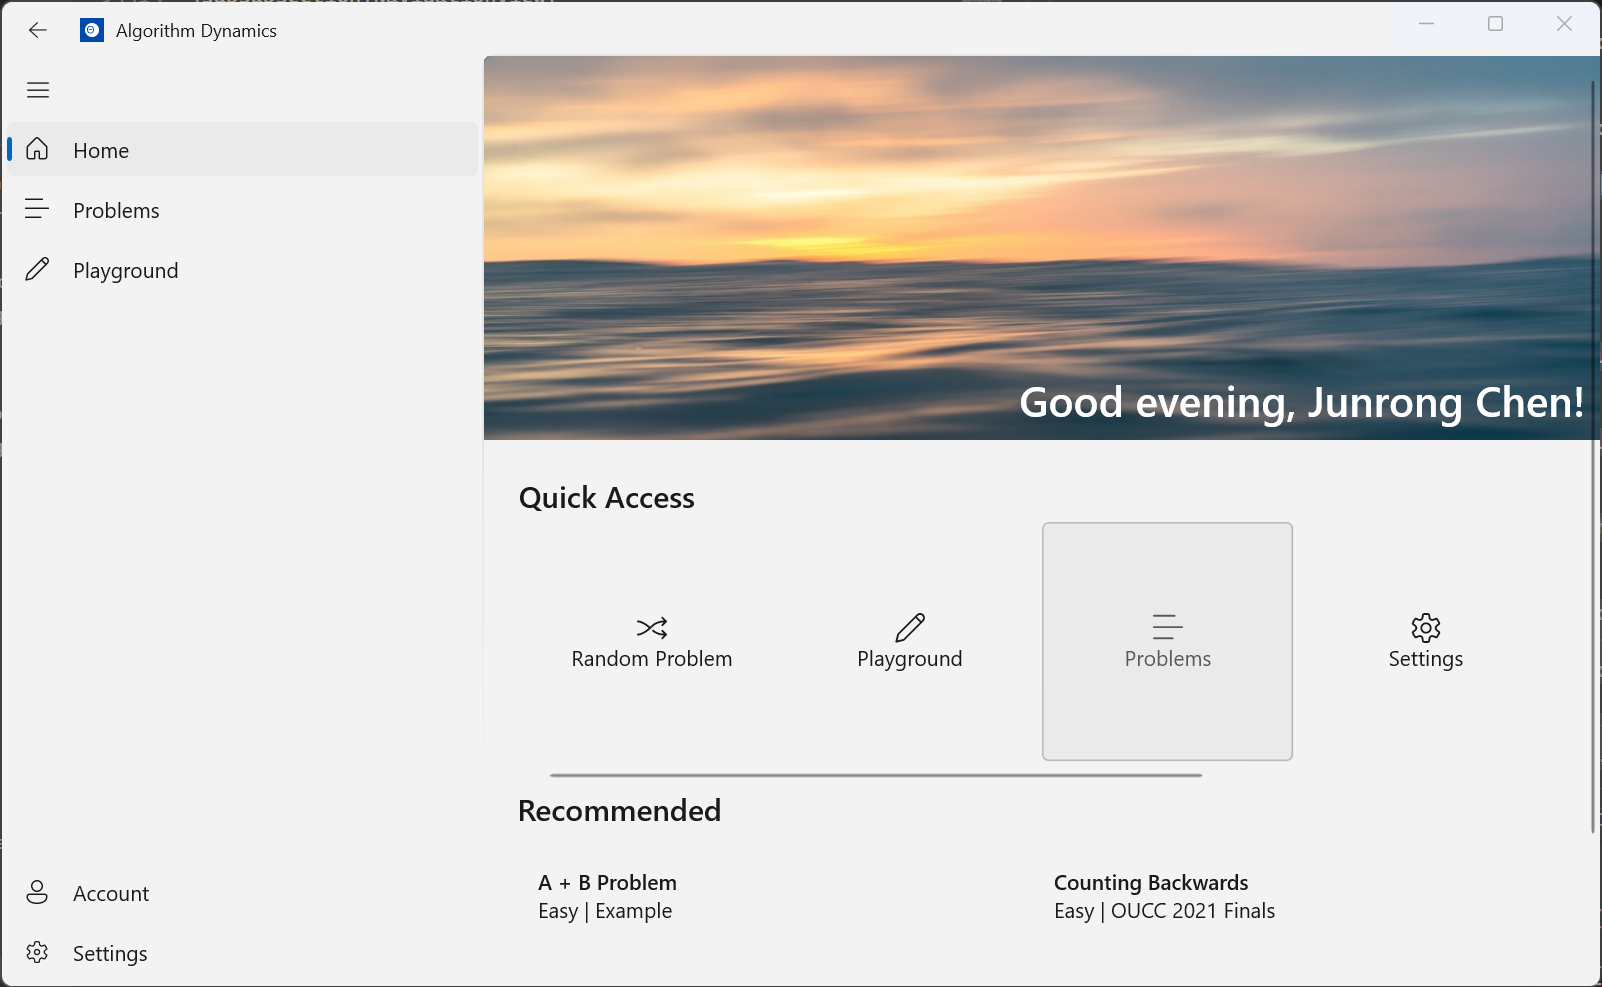
\includegraphics[width=\textwidth, height=\textheight, keepaspectratio]{HomePage-Testing}

\begin{tabulary}{\linewidth}{|L|l|}
    \hline
    Test & Result \\
    \hline
    Does it load & Pass \\
    \hline
    Does the background image show up correctly & Pass \\
    \hline
    Does the greeting message show up correctly & Pass \\
    \hline
    Does the Quick Access Toolbar show up correctly & Pass \\
    \hline
    Does the Quick Access Toolbar work correctly & Pass \\
    \hline
    Does the Recommendation show up correctly & Pass \\
    \hline
    Does the Recommendation work correctly & Pass \\
    \hline
    Is the page responsive & Pass \\
    \hline
\end{tabulary}

\subsubsection{ProblemsPage}

\begin{tabulary}{\linewidth}{|L|l|}
    \hline
    Test & Result \\
    \hline
    Does it load & Pass \\
    \hline
    Does the toolbar display correctly & Pass \\
    \hline
    Does the toolbar interact correctly & Pass \\
    \hline
    Does the toolbar return the correct search result & Pass \\
    \hline
    Does the add button work & Pass \\
    \hline
    Does the problem list show up correct & Pass \\
    \hline
    Does the start button work & Pass \\
    \hline
    Does the selection and menu flyout work & Pass \\
    \hline
\end{tabulary}

Add problem shows up the correct flyout and navigate to the correct page.

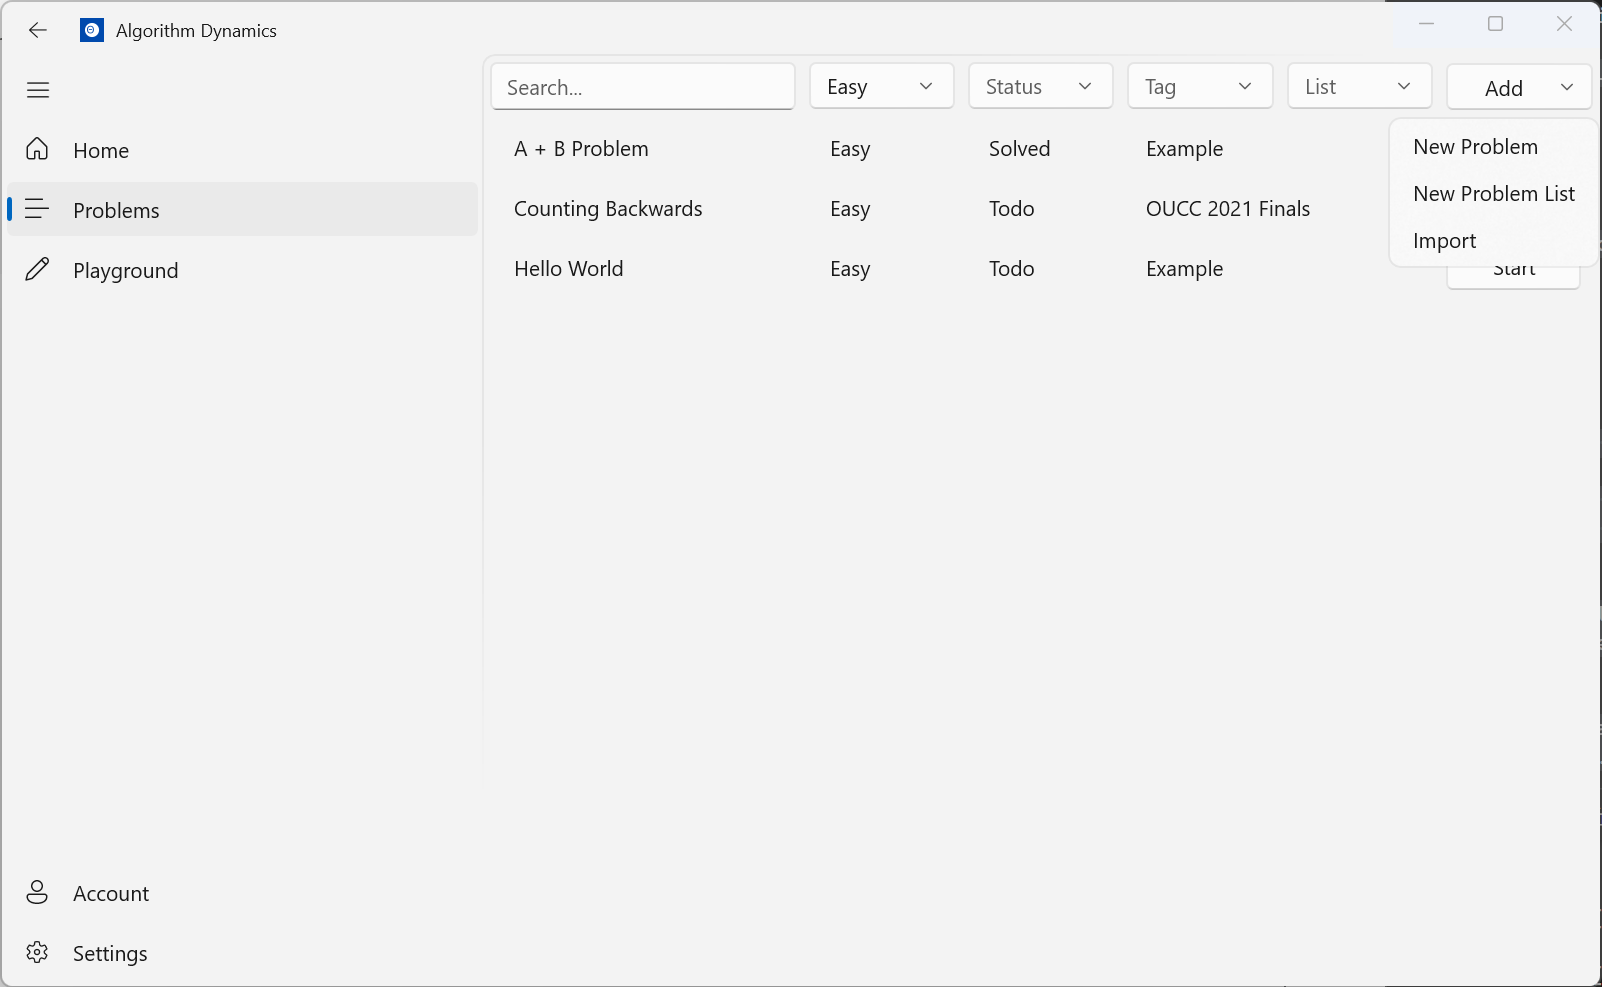
\includegraphics[width=\textwidth, height=\textheight, keepaspectratio]{ProblemsPage-Testing-Add.png}

The right-click flyout menu shows up correctly with all it button functional.

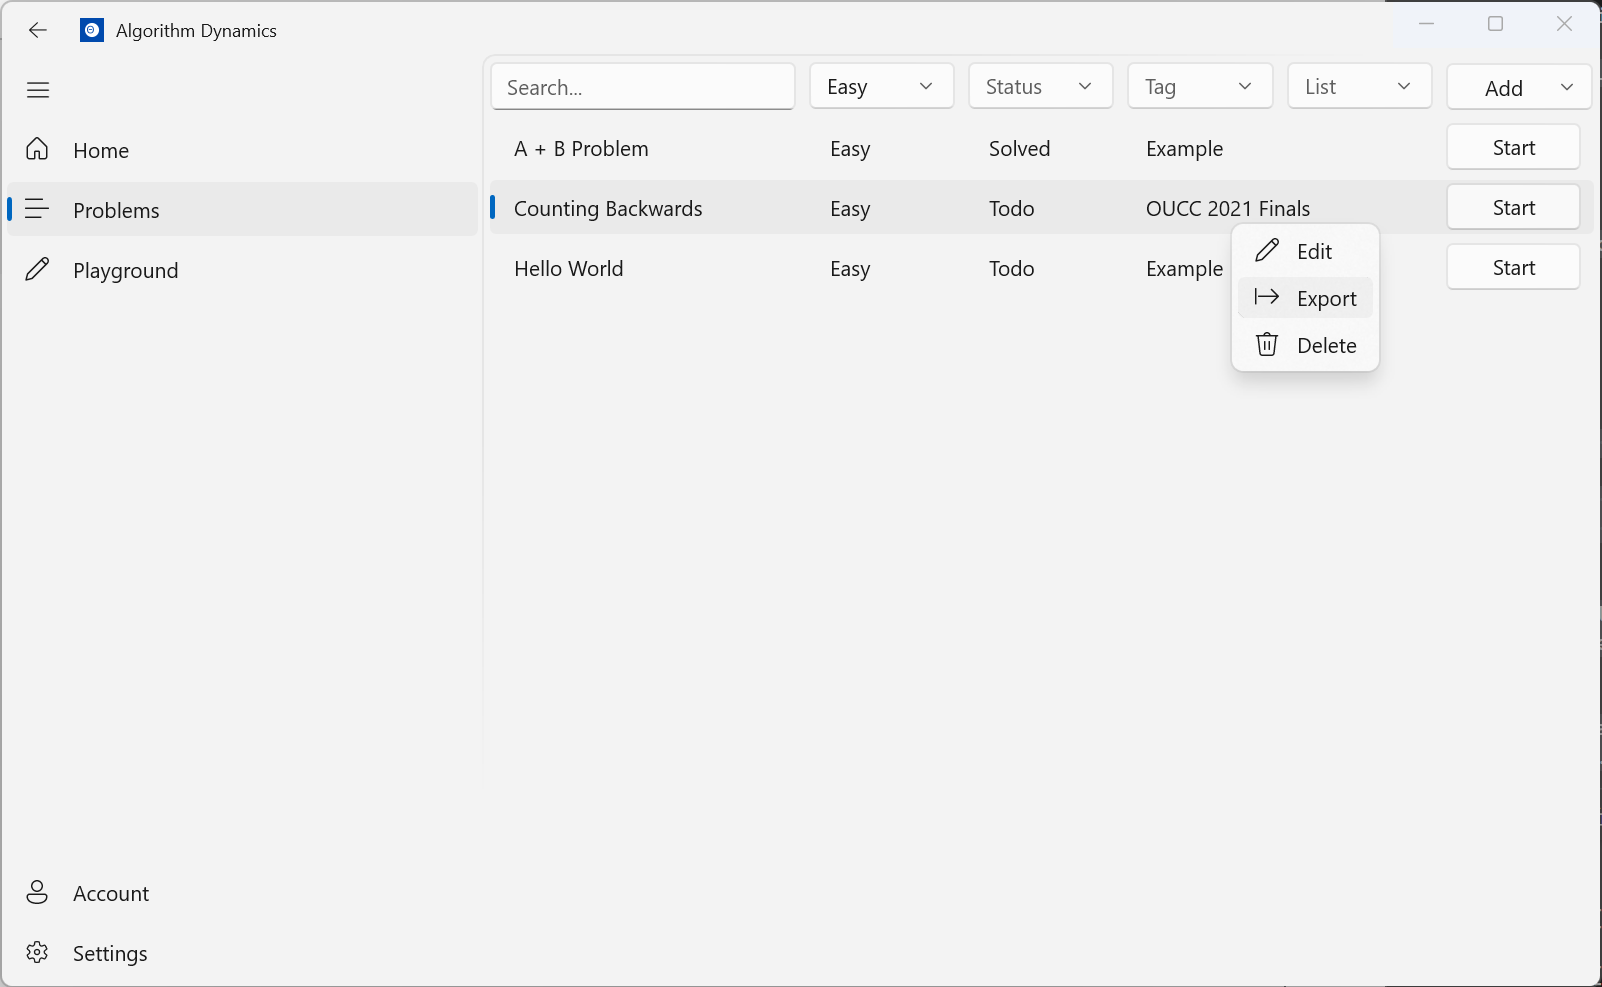
\includegraphics[width=\textwidth, height=\textheight, keepaspectratio]{ProblemsPage-Testing-Flyout.png}

The file picker shows up correctly and the problems or problem lists are imported correctly.

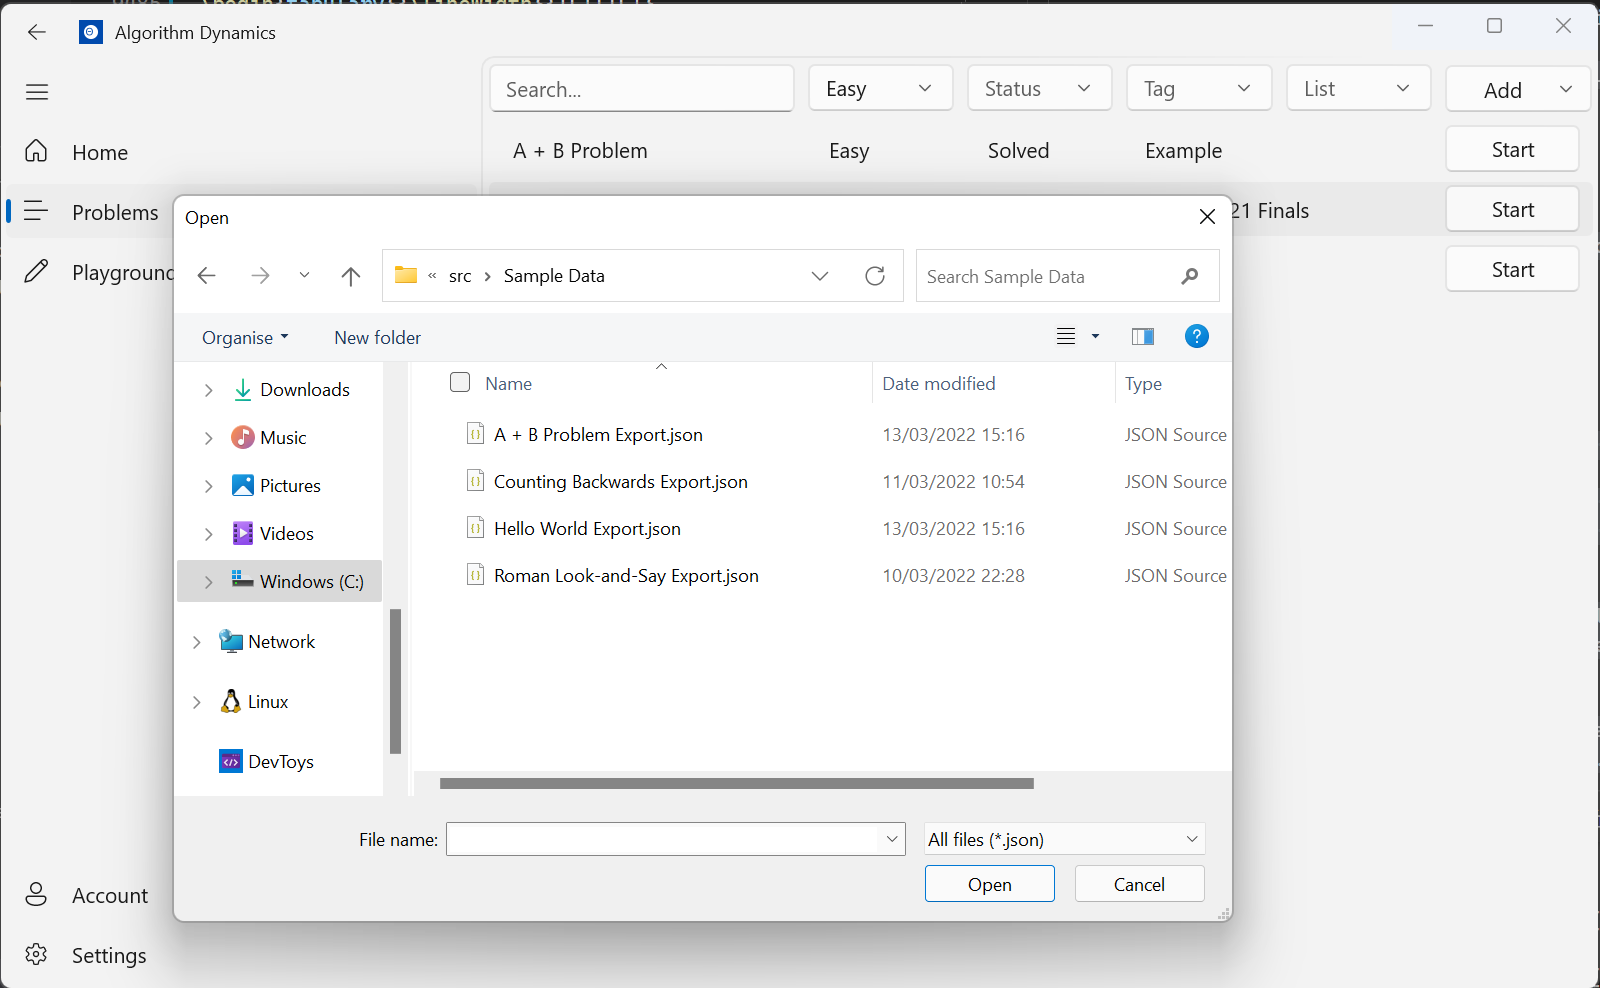
\includegraphics[width=\textwidth, height=\textheight, keepaspectratio]{ProblemsPage-Testing-Import.png}

The search bar is fully functional.

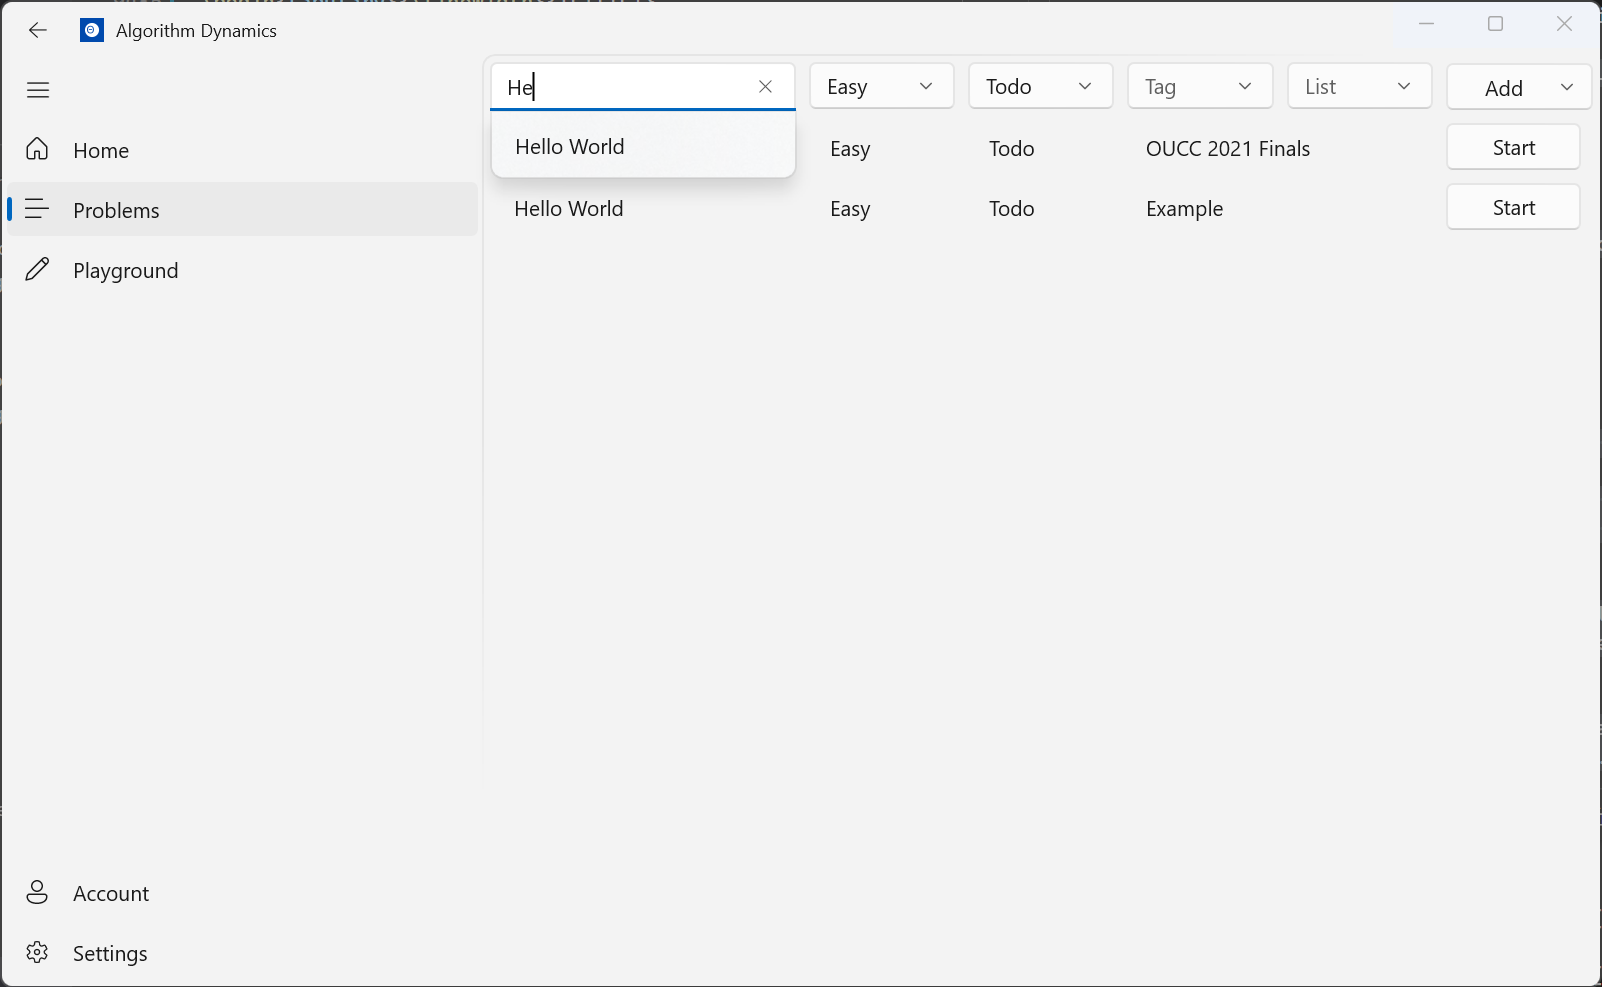
\includegraphics[width=\textwidth, height=\textheight, keepaspectratio]{ProblemsPage-Testing-Search.png}

\subsubsection{CreateNewProblemPage}

\begin{tabulary}{\linewidth}{|L|l|}
    \hline
    Test & Result \\
    \hline
    Does it load & Pass \\
    \hline
    Does the title field work & Pass \\
    \hline
    Does the tags field work & Pass \\
    \hline
    Does the difficulty field work & Pass \\
    \hline
    Does the time limit field work and validate the data & Pass \\
    \hline
    Does the memory limit field work and validate the data & Pass \\
    \hline
    Does the description field work & Pass \\
    \hline
    Does the preview block work & Pass \\
    \hline
    Is it possible to add or remove test cases & Pass \\
    \hline
    Does the cancel button work & Pass \\
    \hline
    Does the save button work & Pass \\
    \hline
\end{tabulary}

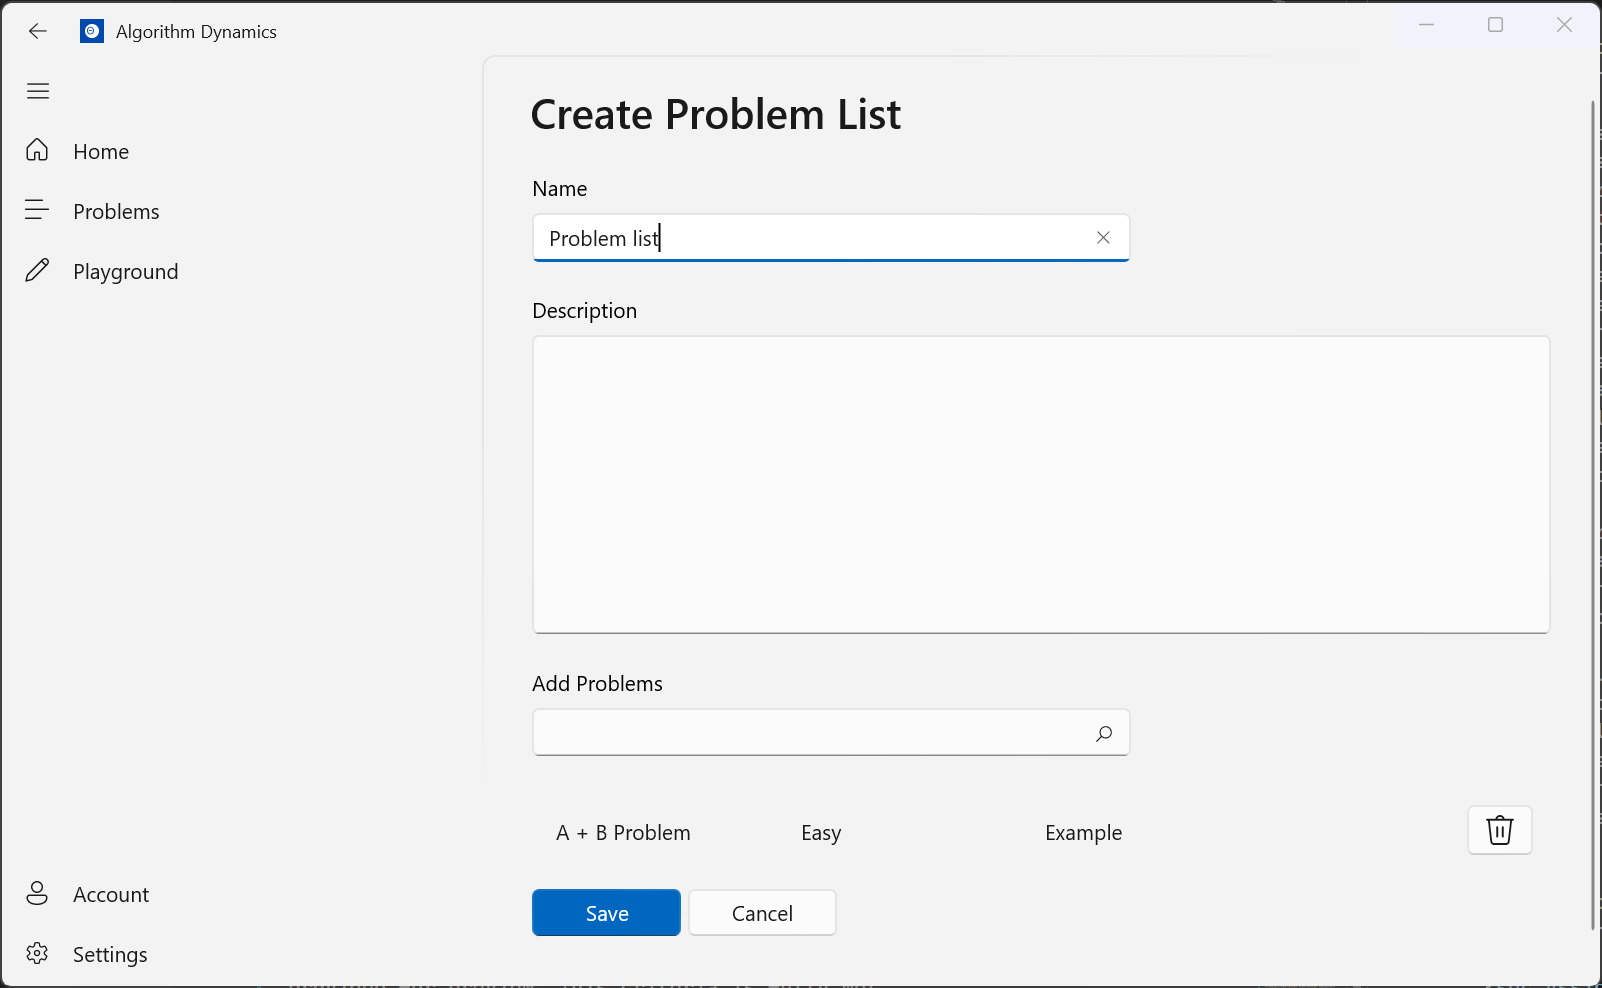
\includegraphics[width=\textwidth, height=\textheight, keepaspectratio]{CreateNewProblemListPage-Final}

\subsubsection{CreateNewProblmeListPage}

\begin{tabulary}{\linewidth}{|L|l|}
    \hline
    Does it load & Pass \\
    \hline
    Does the title field work & Pass \\
    \hline
    Does the description field work & Pass \\
    \hline
    Does the search box work & Pass \\
    \hline
    Does the cancel button work & Pass \\
    \hline
    Does the save button work & Pass \\
    \hline
    Does the export button work & Pass \\
    \hline
\end{tabulary}

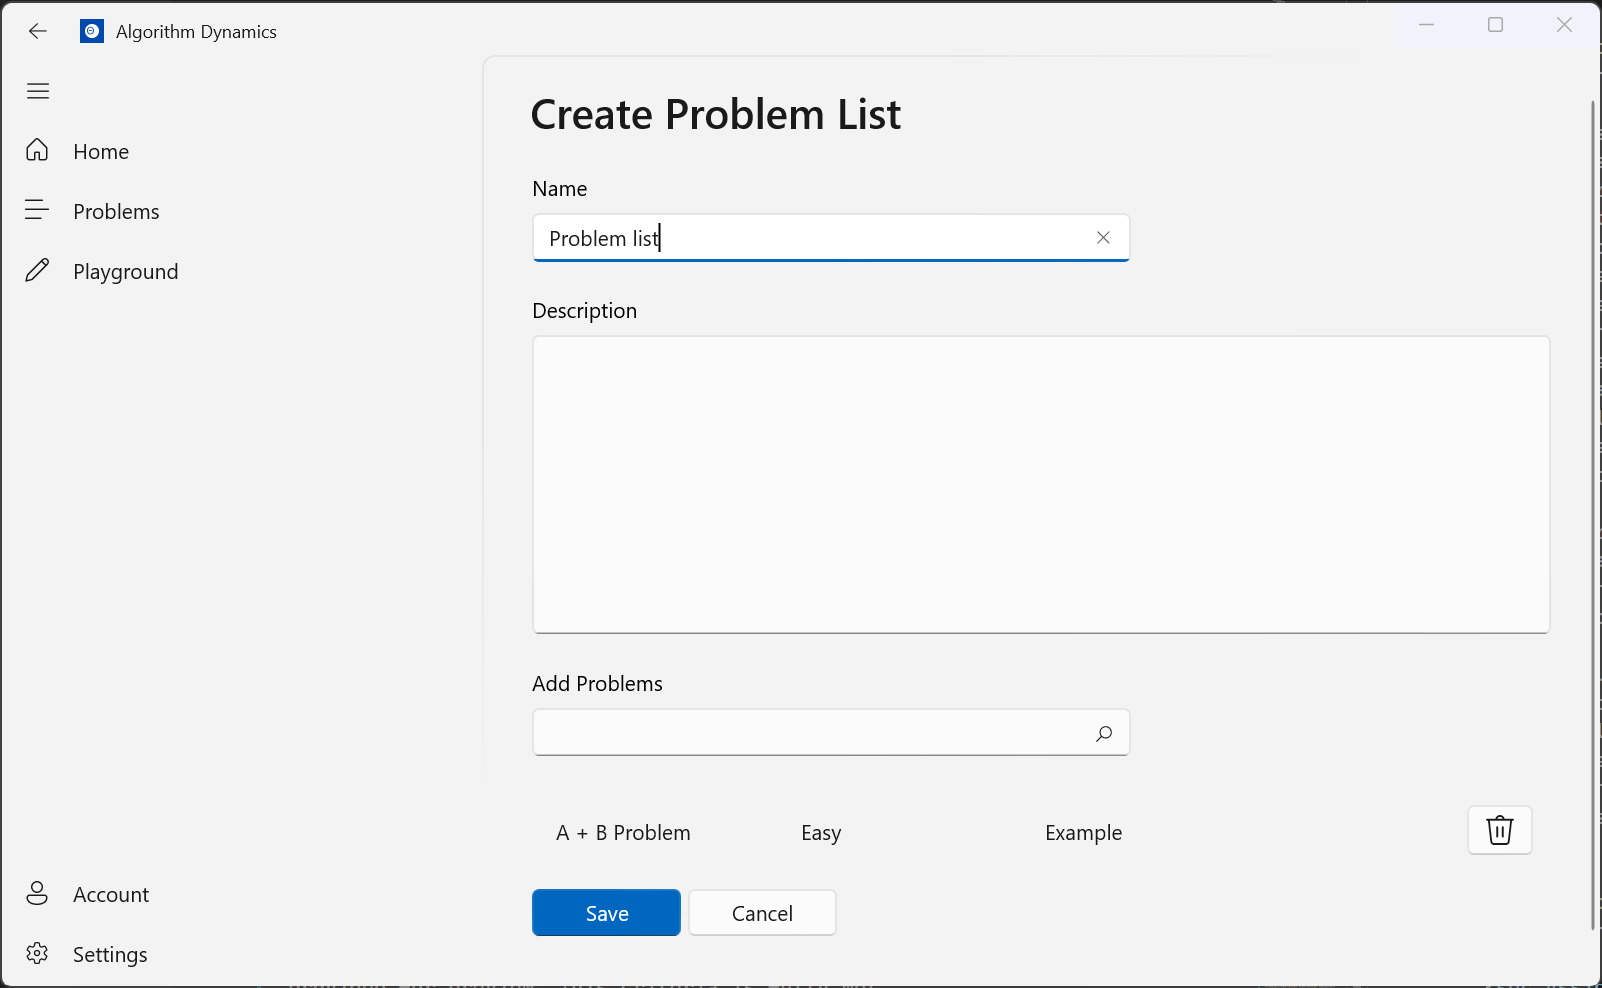
\includegraphics[width=\textwidth, height=\textheight, keepaspectratio]{CreateNewProblemListPage-Final}

\subsubsection{CodingPage}

\begin{tabulary}{\linewidth}{|L|l|}
    \hline
    Test & Result \\
    \hline
    Does it load & Pass \\
    \hline
    Does the full screen button work & Pass \\
    \hline
    Does the markdown text block work & Pass \\
    \hline
    Does the code editor work & Pass \\
    \hline
    Does the input panel work & Pass \\
    \hline
    Does the output panel work & Pass \\
    \hline
    Does the error panel work & Pass \\
    \hline
    Does the language selection box work & Pass \\
    \hline
    Does the Run Code button work & Pass \\
    \hline
    Does the Submit button work & Pass \\
    \hline
    Does the Submit problem navigation & Pass \\
    \hline
    Does the submission history table work & Pass \\
    \hline
\end{tabulary}

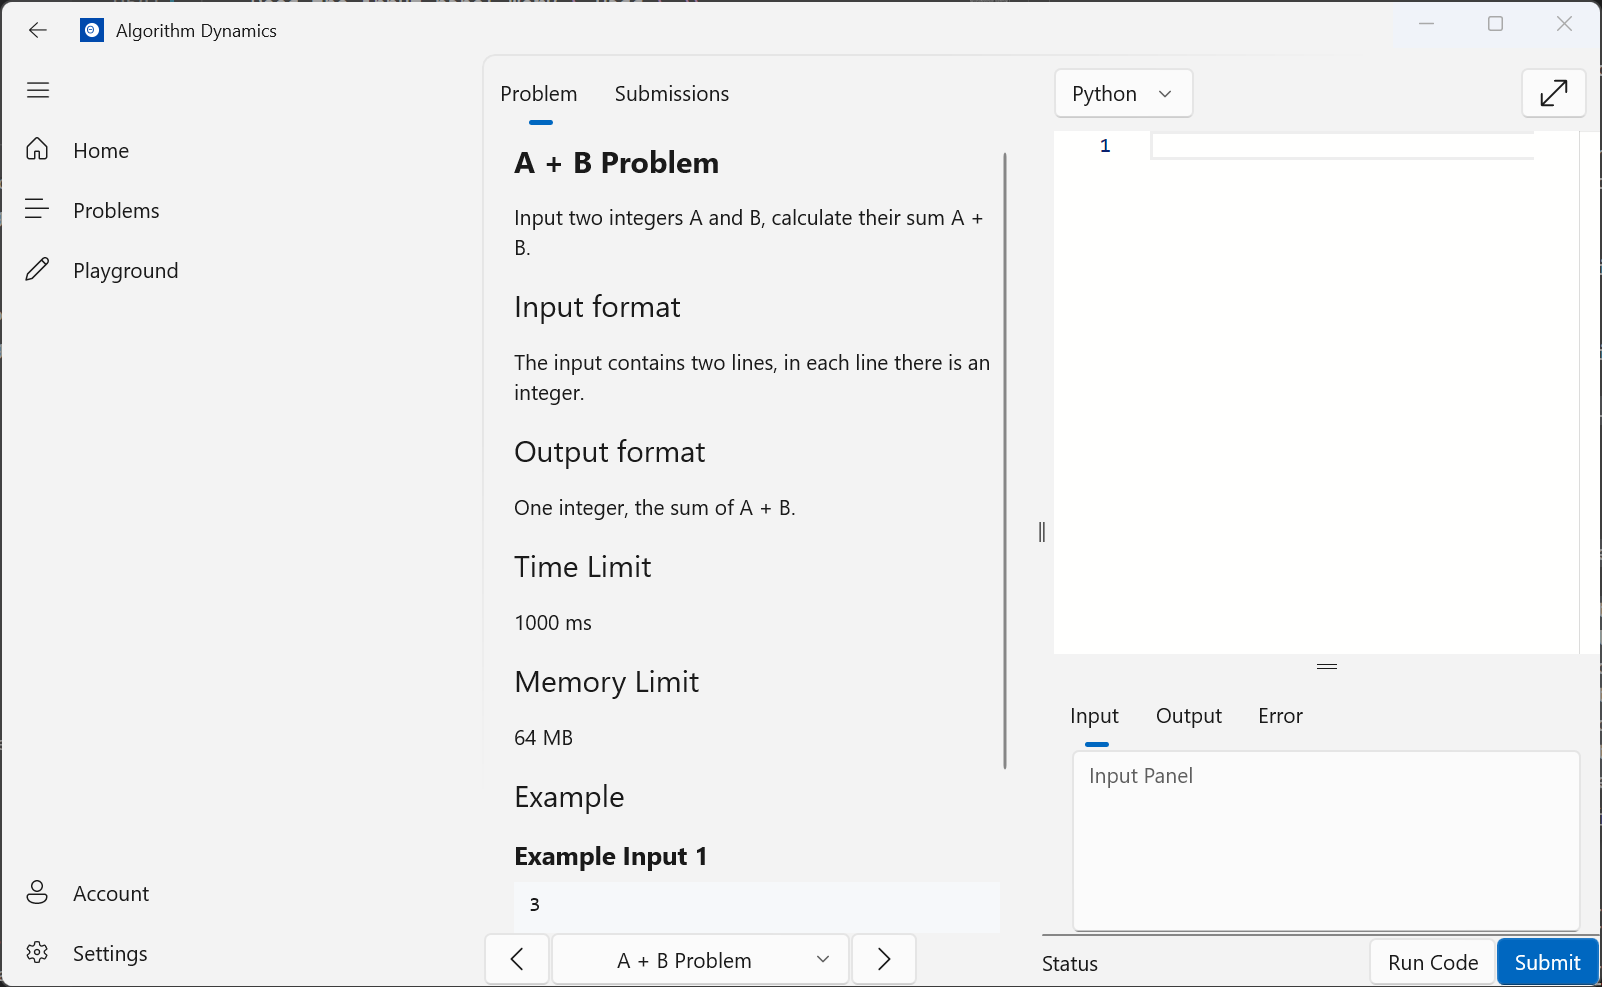
\includegraphics[width=\textwidth, height=\textheight, keepaspectratio]{CodingPage-Testing}

The RunCode button runs the code against the given input correctly. 

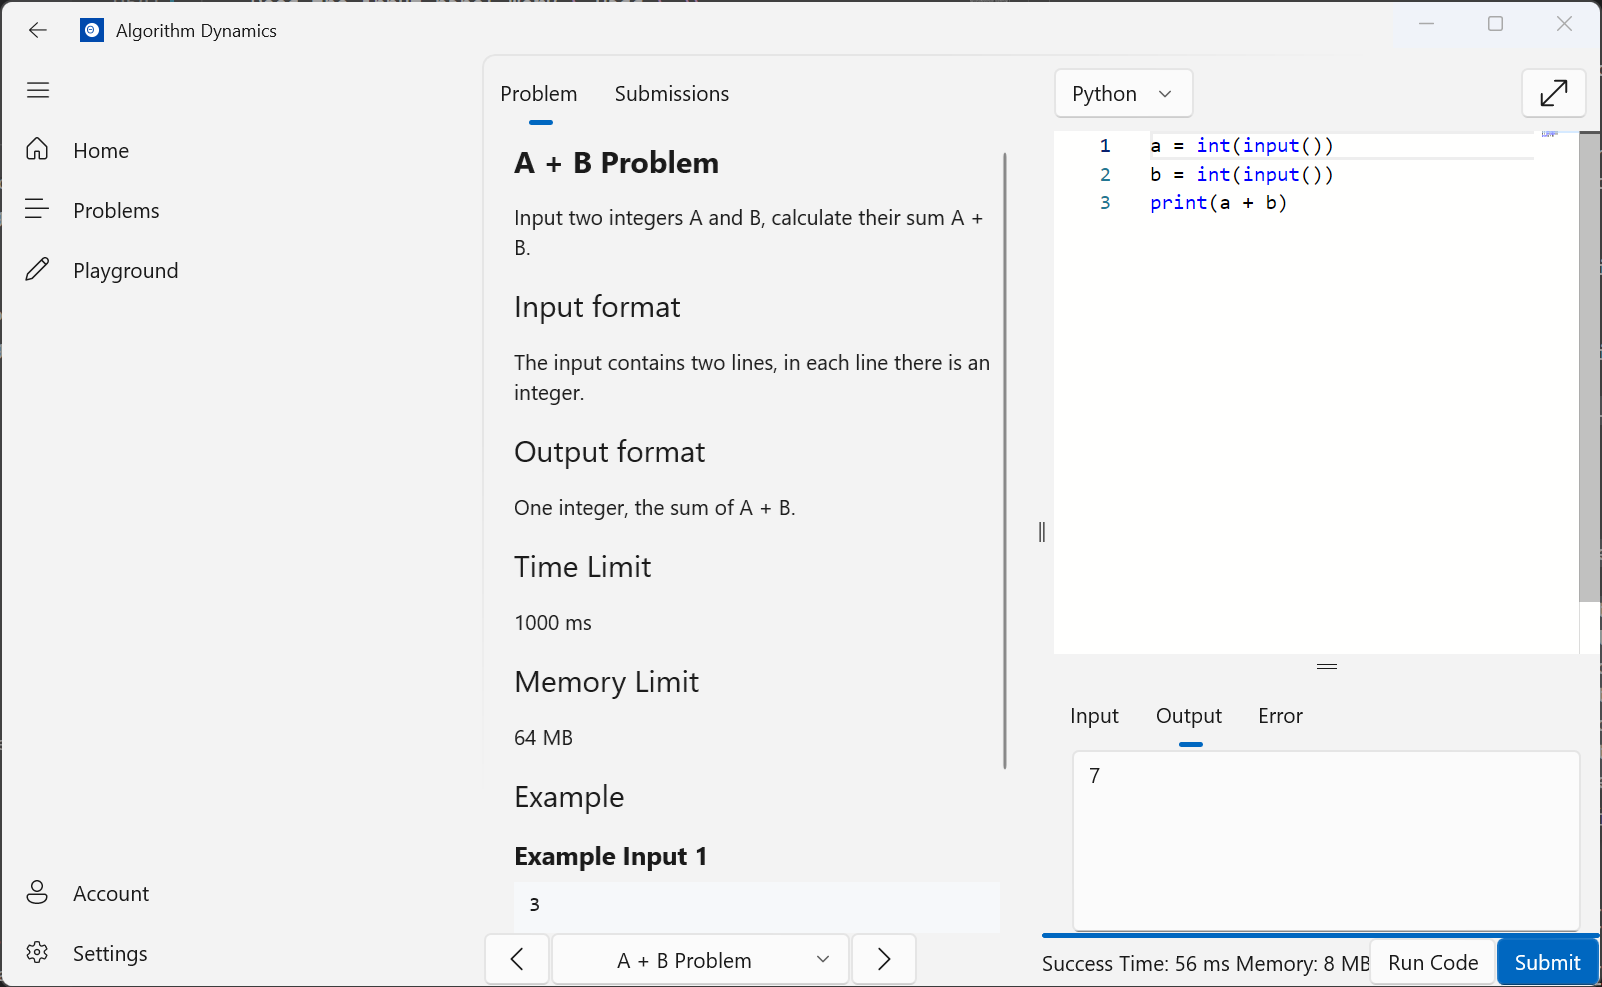
\includegraphics[width=\textwidth, height=\textheight, keepaspectratio]{CodingPage-Testing-RunCode}

The Submission button submits the code for judging and save the result to the database correctly.

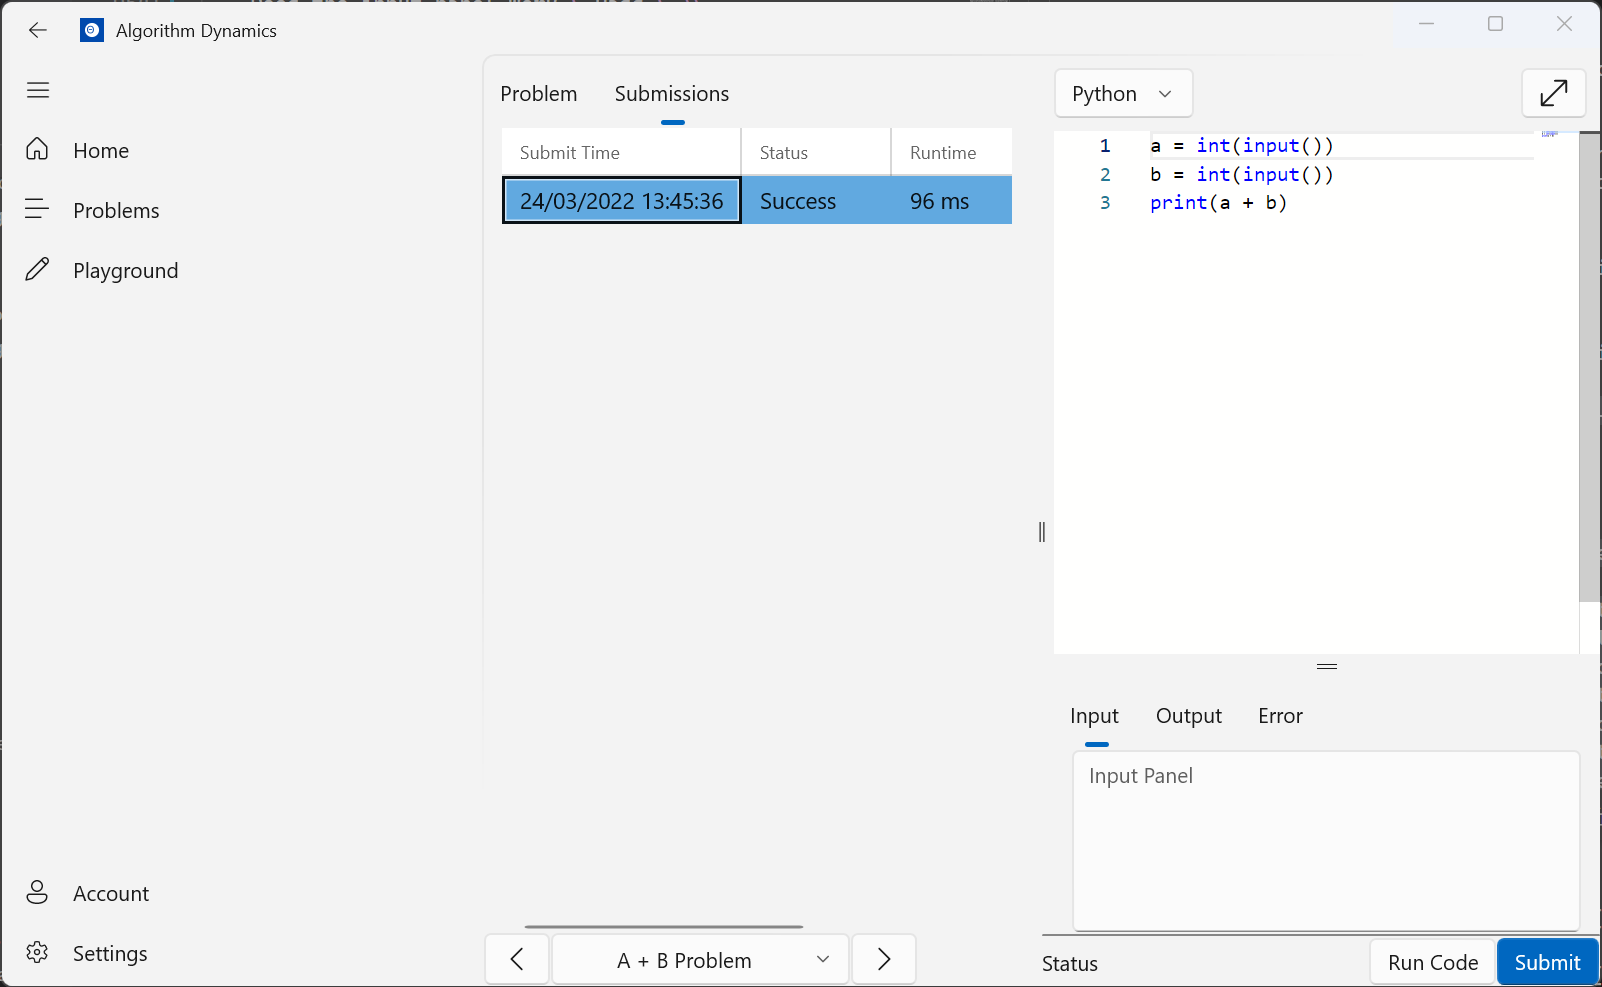
\includegraphics[width=\textwidth, height=\textheight, keepaspectratio]{CodingPage-Testing-Submission}

The navigation menu switches between different problems correctly.

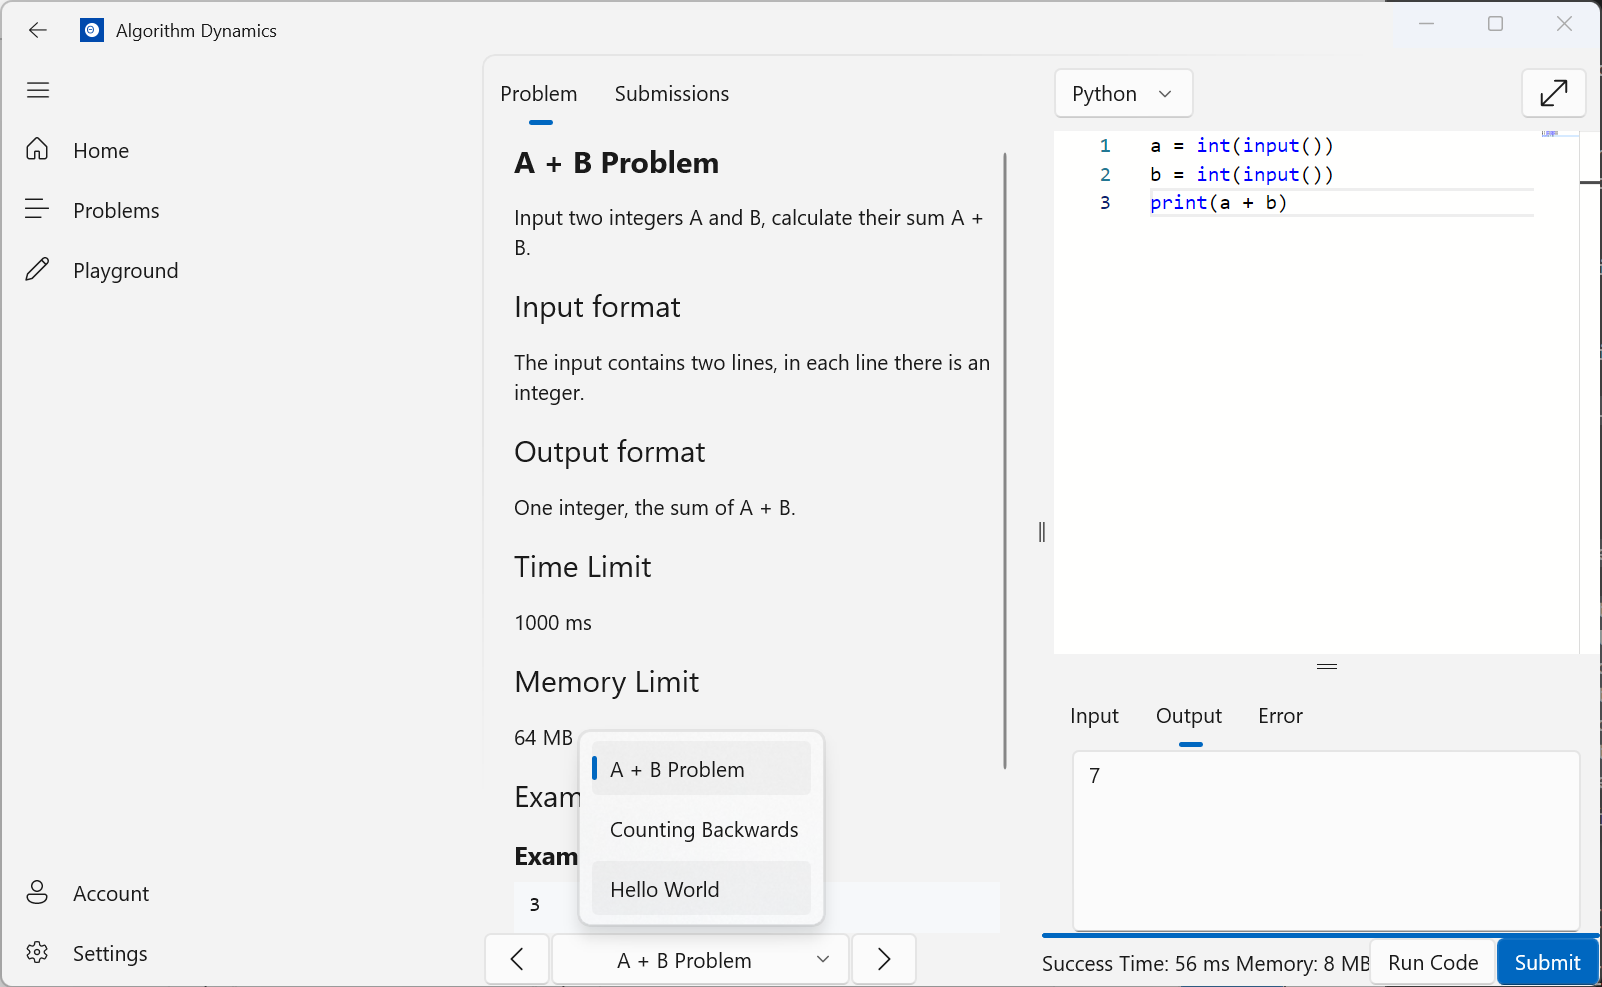
\includegraphics[width=\textwidth, height=\textheight, keepaspectratio]{CodingPage-Testing-Navigation}

The programming language selection box switches between different languages in runtime correctly.

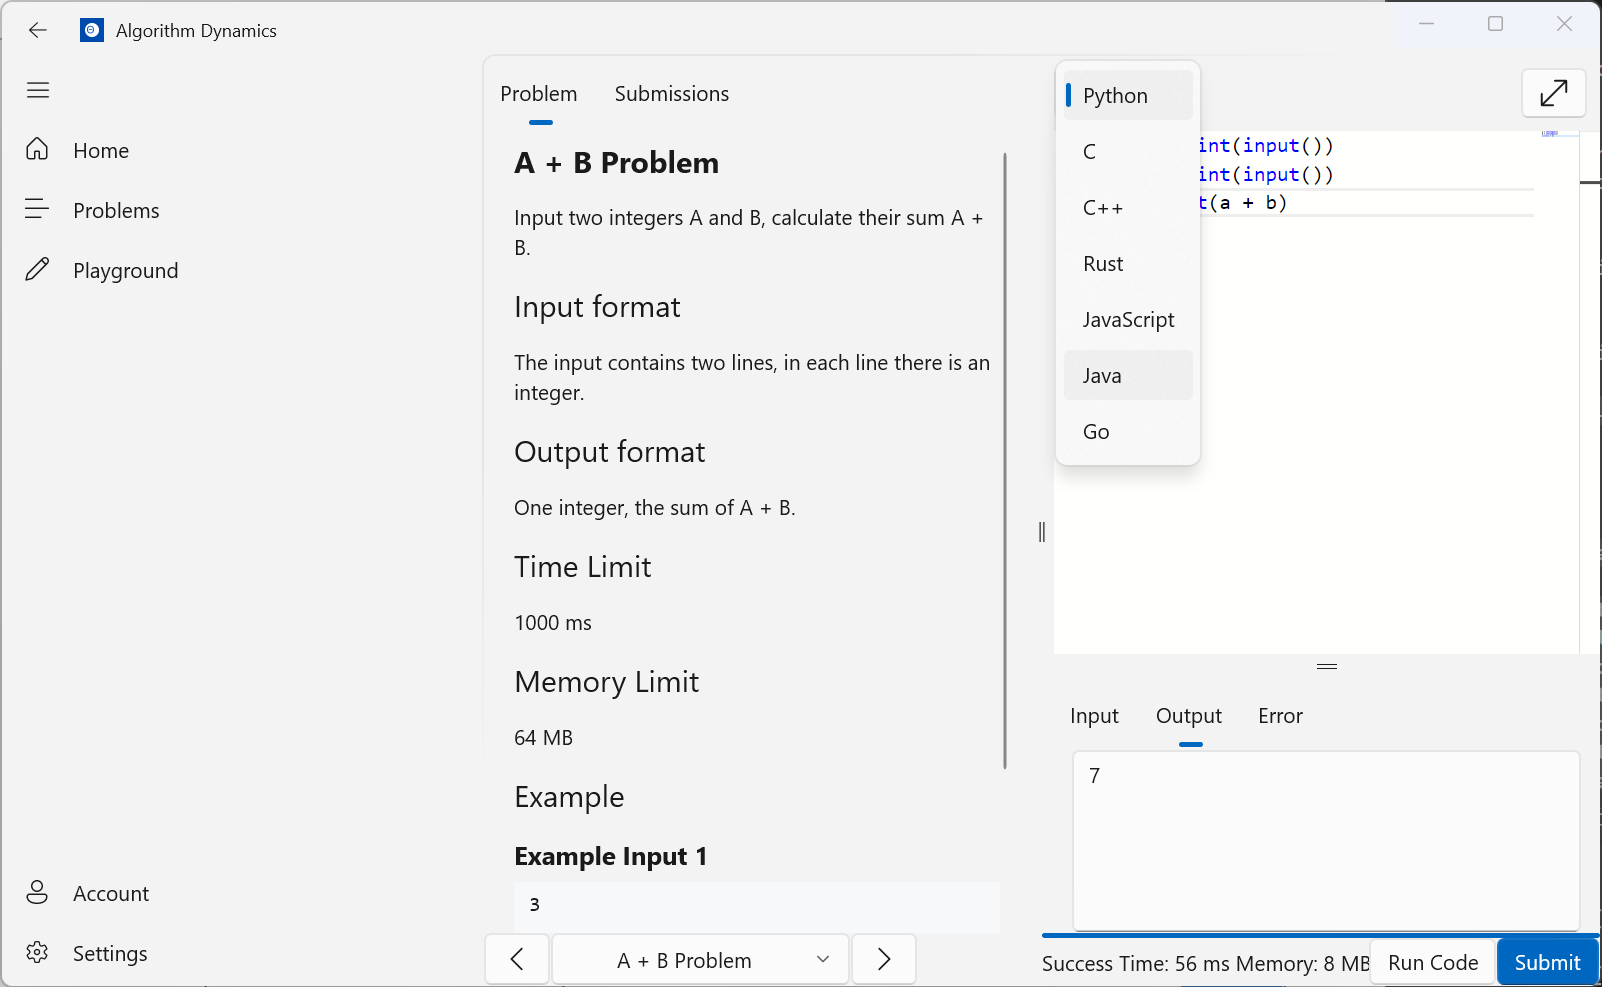
\includegraphics[width=\textwidth, height=\textheight, keepaspectratio]{CodingPage-Testing-Language}

\subsubsection{PlaygroundPage}

\begin{tabulary}{\linewidth}{|L|l|}
    \hline
    Test & Result \\
    \hline
    Does it load & Pass \\
    \hline
    Can each section be resized correctly & Pass \\
    \hline
    Does the CodeEditor work correctly & Pass \\
    \hline
    Does the language ComboBox work correctly & Pass \\
    \hline
    Does the input output box work correctly & Pass \\
    \hline
    Does the Run Code button work & Pass \\
    \hline
    Is the CodeEditor unloaded correctly on close & Pass \\
    \hline
\end{tabulary}

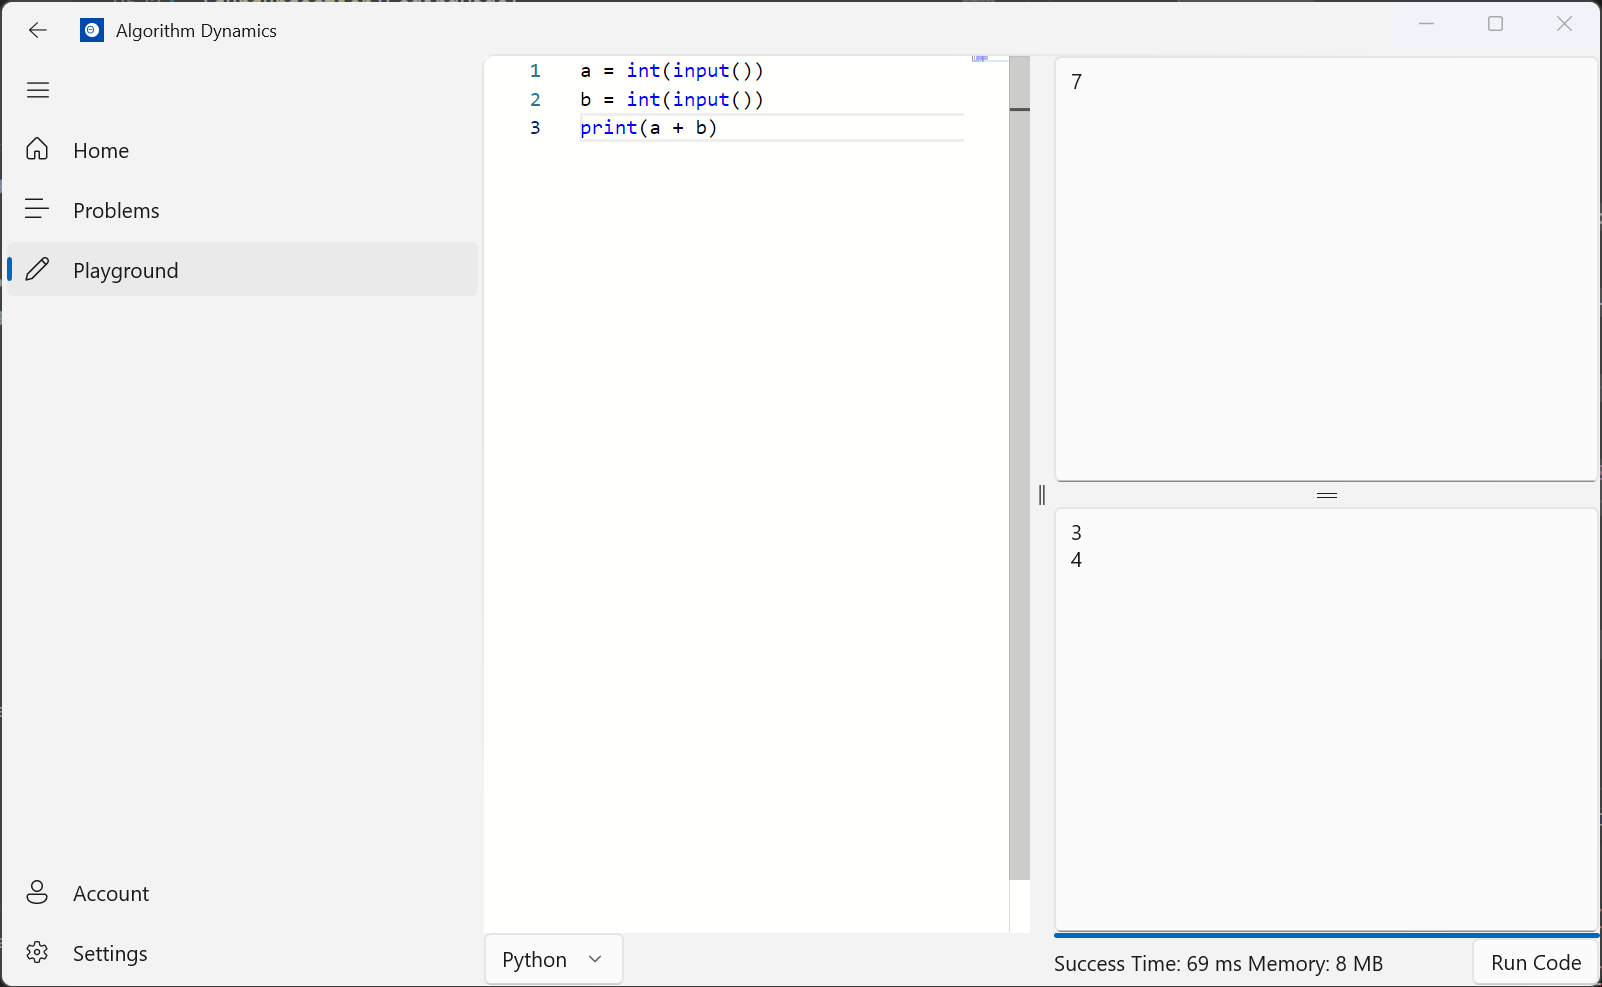
\includegraphics[width=\textwidth, height=\textheight, keepaspectratio]{PlaygroundPage-Testing}

\subsubsection{AccountPage}

\begin{tabulary}{\linewidth}{|L|l|}
    \hline
    Test & Result\\
    \hline
    Does it load & Pass \\
    \hline
    Does the Edit button work & Pass \\
    \hline
    Does the statistics data show up correctly & Pass \\
    \hline
\end{tabulary}

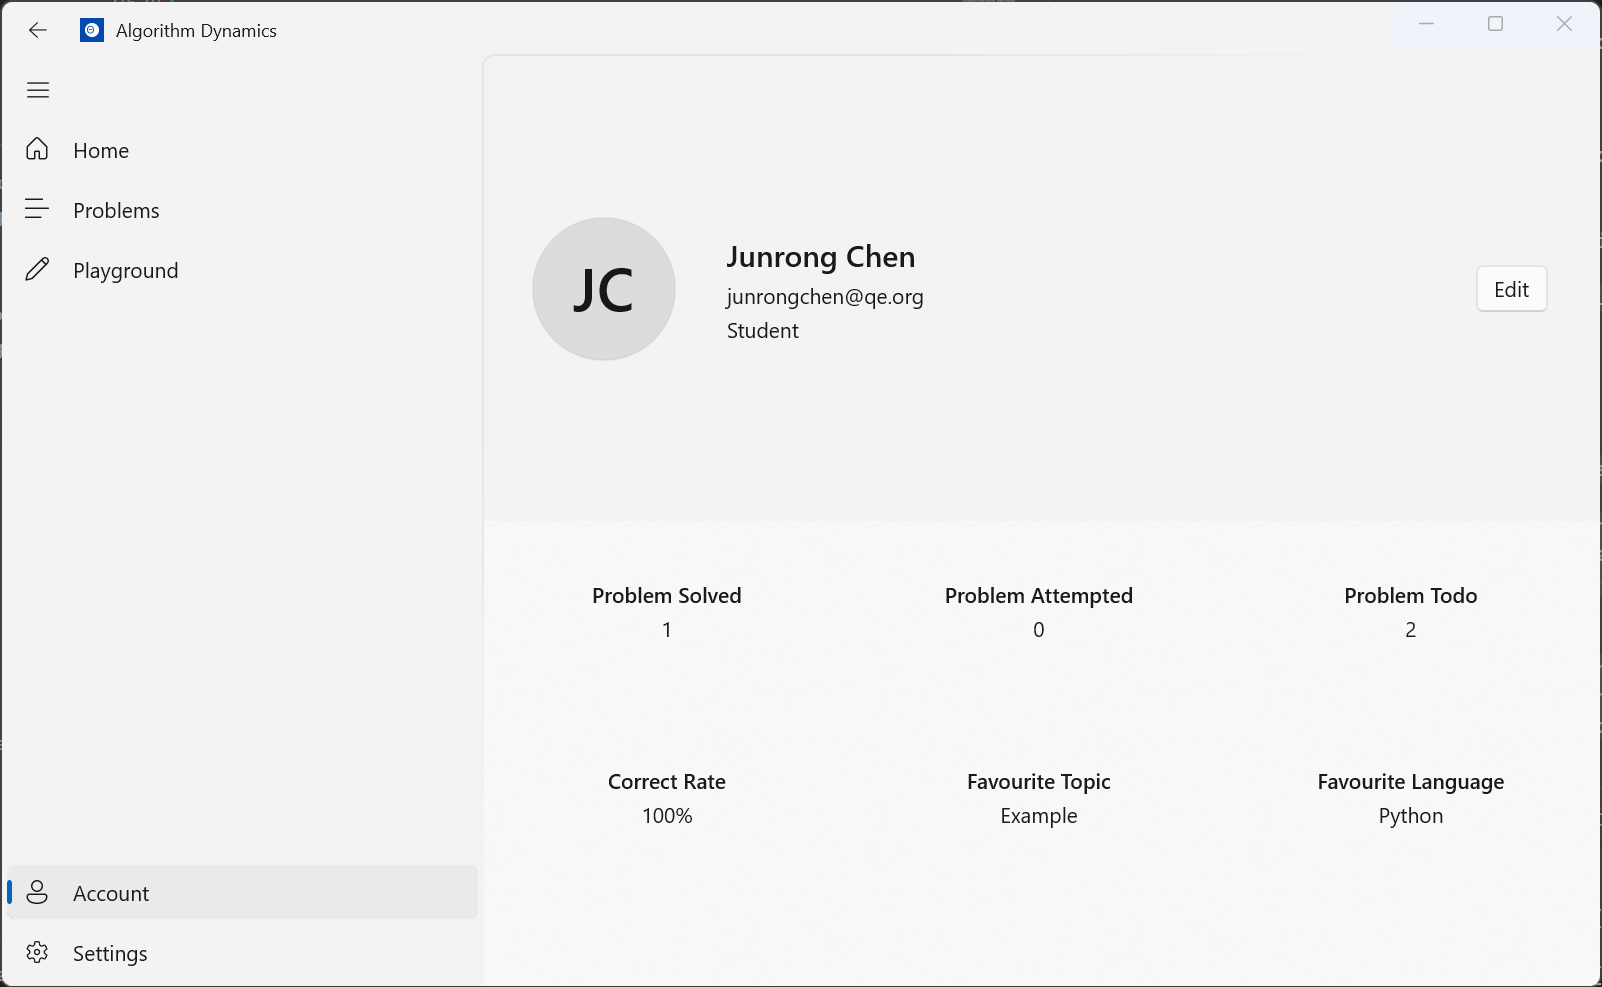
\includegraphics[width=\textwidth, height=\textheight, keepaspectratio]{AccountPage-Testing}

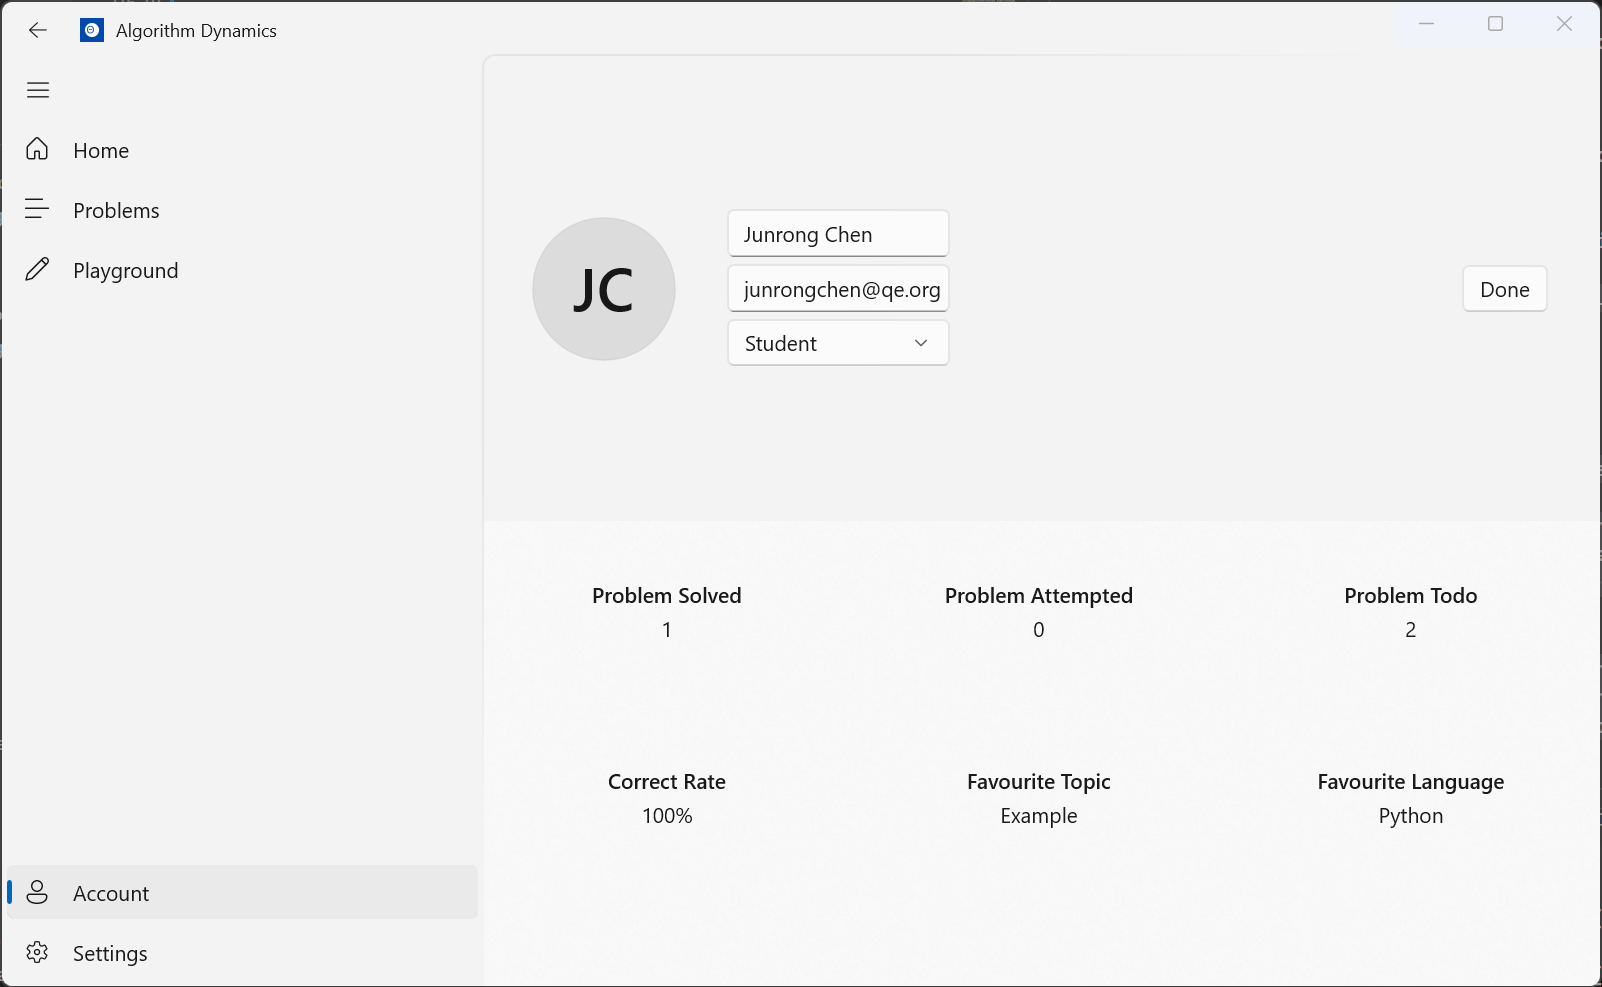
\includegraphics[width=\textwidth, height=\textheight, keepaspectratio]{AccountPage-Testing-Edit}

\subsubsection{SettingsPage}

\begin{tabulary}{\linewidth}{|L|l|}
    \hline
    Does it load & Pass \\
    \hline
    Does theme switch work & Pass \\
    \hline
    Does the run code time limit field work and validate the data & Pass \\
    \hline
    Does the run code memory limit field work and validate the data & Pass \\
    \hline
    Does the language configuration editor works & Pass \\
    \hline
    Does the about buttons work & Pass \\
    \hline
    Does the settings get loaded and saved correctly & Pass \\
    \hline
\end{tabulary}

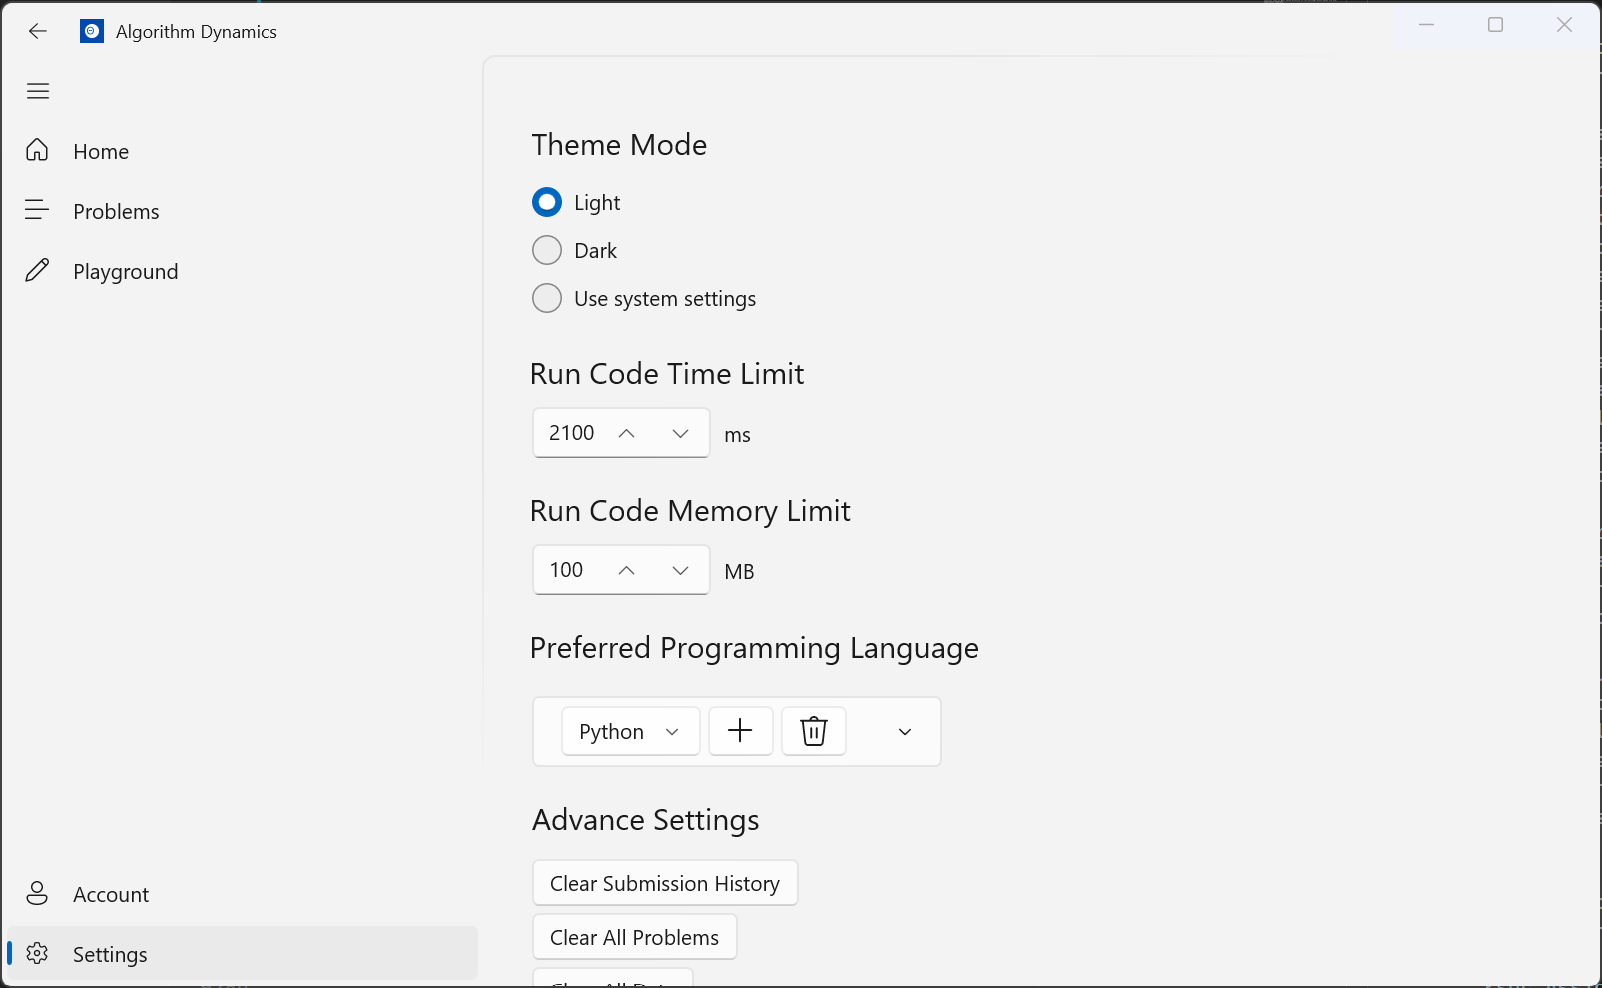
\includegraphics[width=\textwidth, height=\textheight, keepaspectratio]{SettingsPage-Final}

\subsection{Robustness testing}

\subsubsection{ProblemsPage}

Empty search: Pass

An empty string is passed to the search box. The search box returns all problems which are as expected.

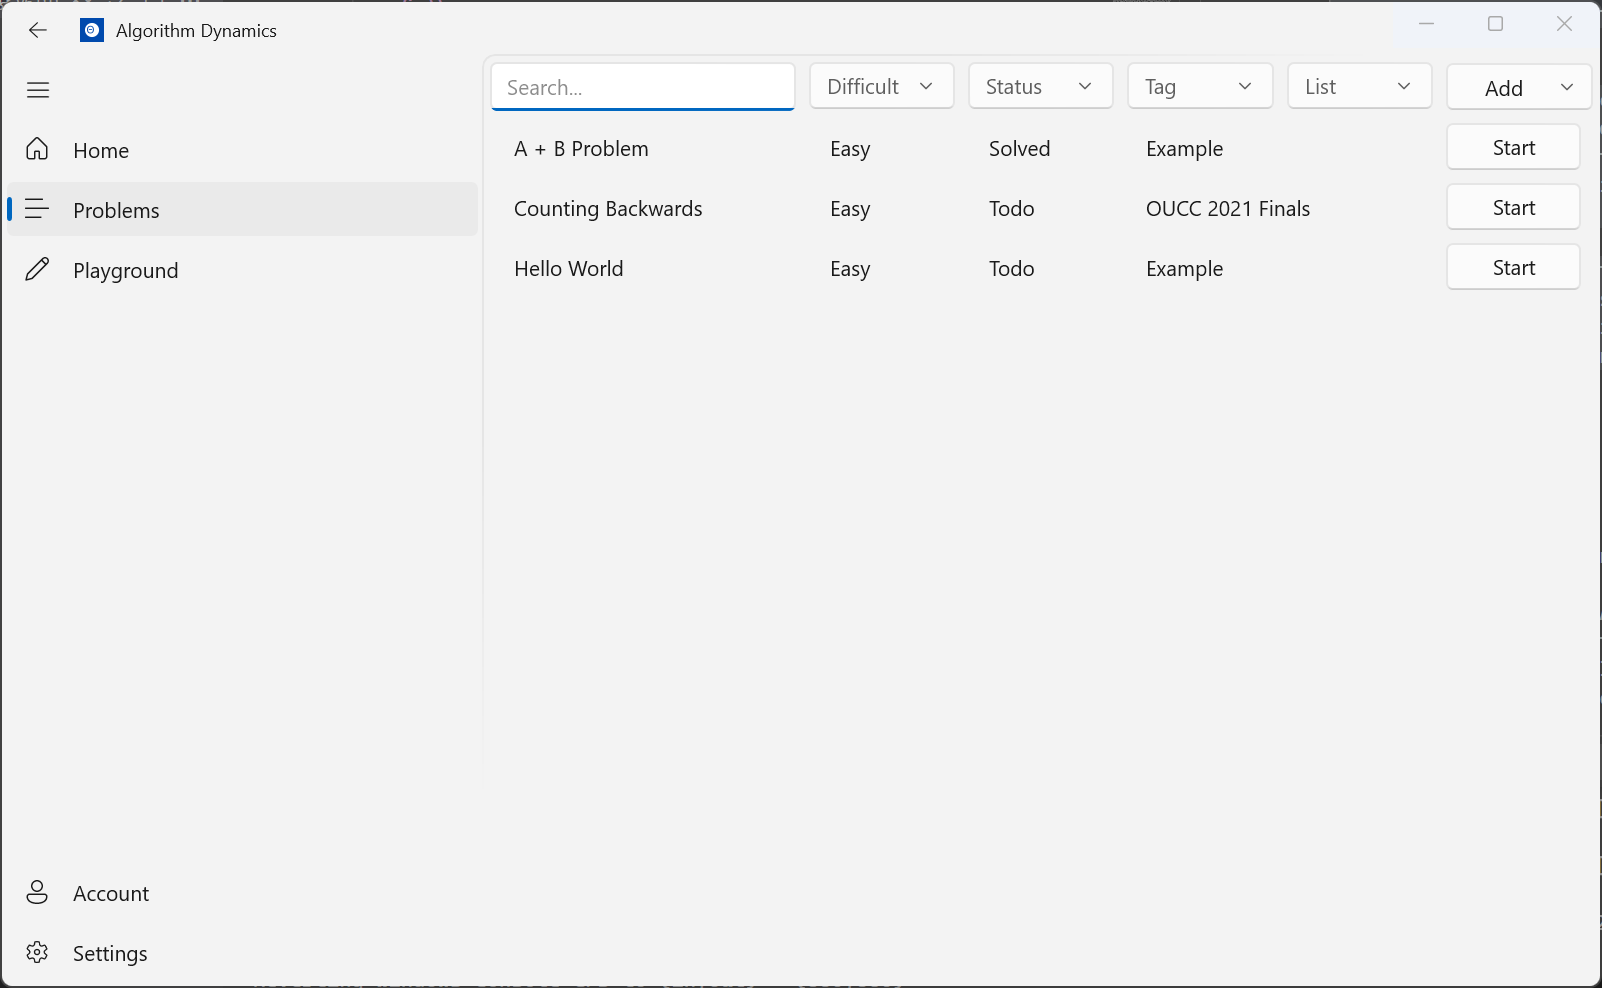
\includegraphics[width=\textwidth, height=\textheight, keepaspectratio]{ProblemsPage-Testing-EmptySearch}

Not exist search: Pass

A non-existing problem name is passed to the search box. The search box returns the correct error message.

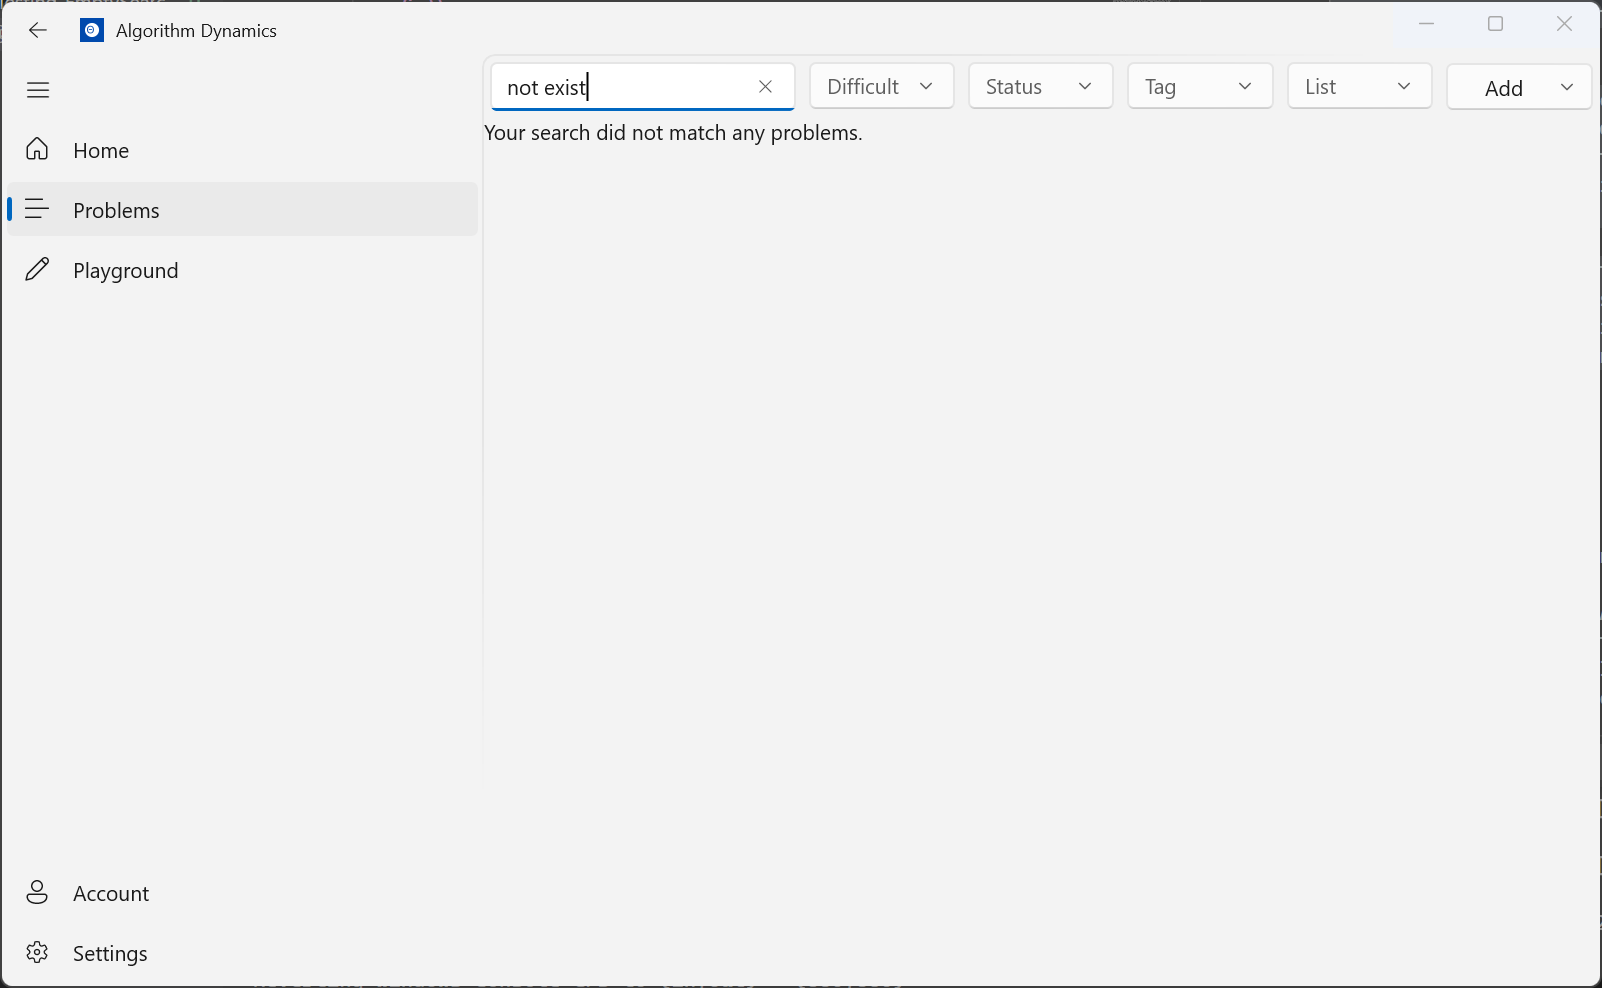
\includegraphics[width=\textwidth, height=\textheight, keepaspectratio]{ProblemsPage-Testing-NotExist}

Wrong import file: Pass

A non-correct import file is passed to the import button. The import button returns the correct error message.

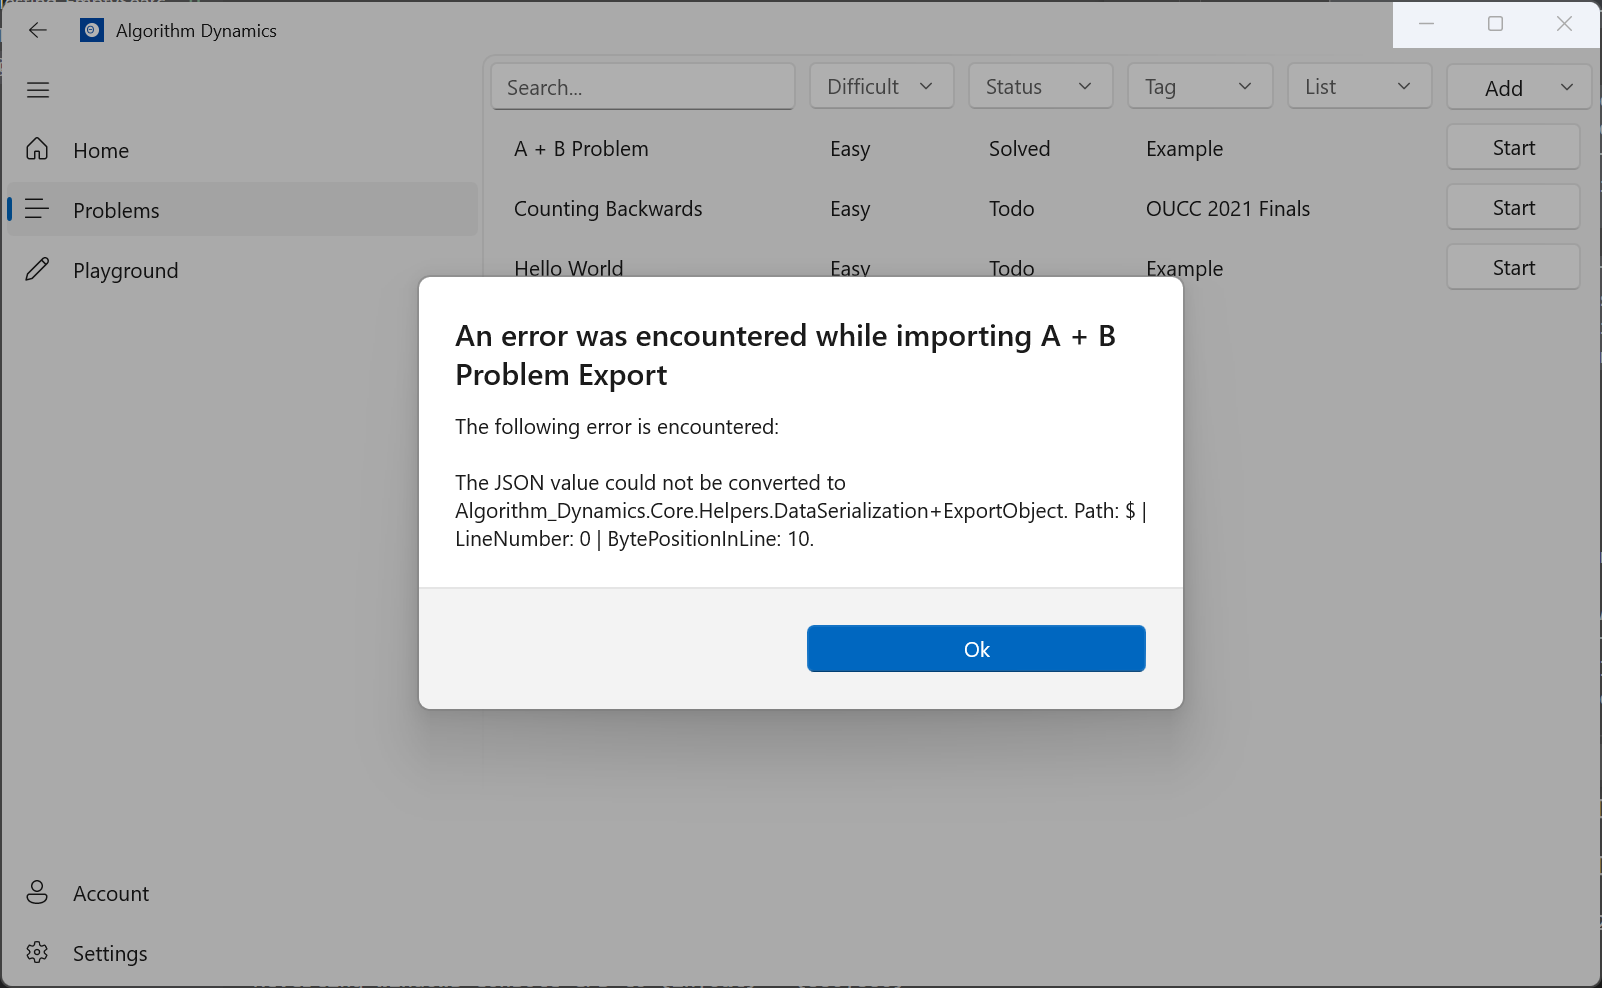
\includegraphics[width=\textwidth, height=\textheight, keepaspectratio]{ProblemsPage-Testing-ImportInvalid}

\subsubsection{CreateNewProblmePage}

Empty input: Pass

No name or test case is input, the save button is disabled and a correct error message is displayed.

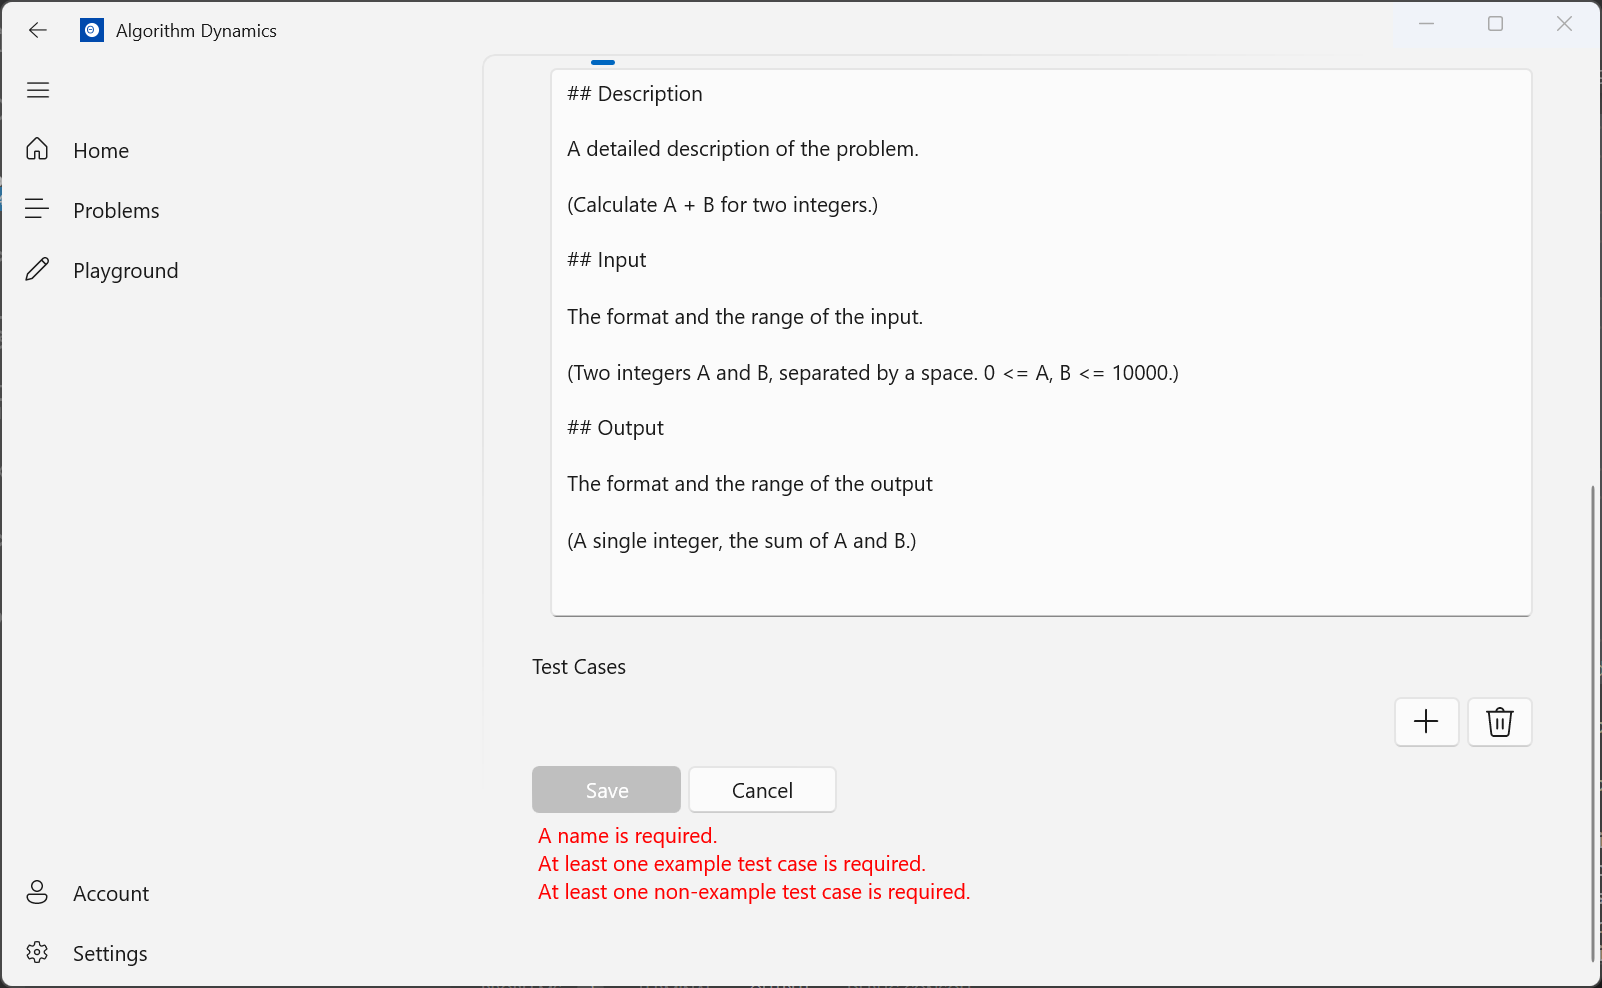
\includegraphics[width=\textwidth, height=\textheight, keepaspectratio]{CreateNewProblemPage-Testing-Empty}

Invalid input: Pass

Invalid input gets filtered by the controls automatically.

\subsubsection{CreateNewProblmeListPage}

Empty input: Pass

No name is input, the save button is disabled and a correct error message is displayed.

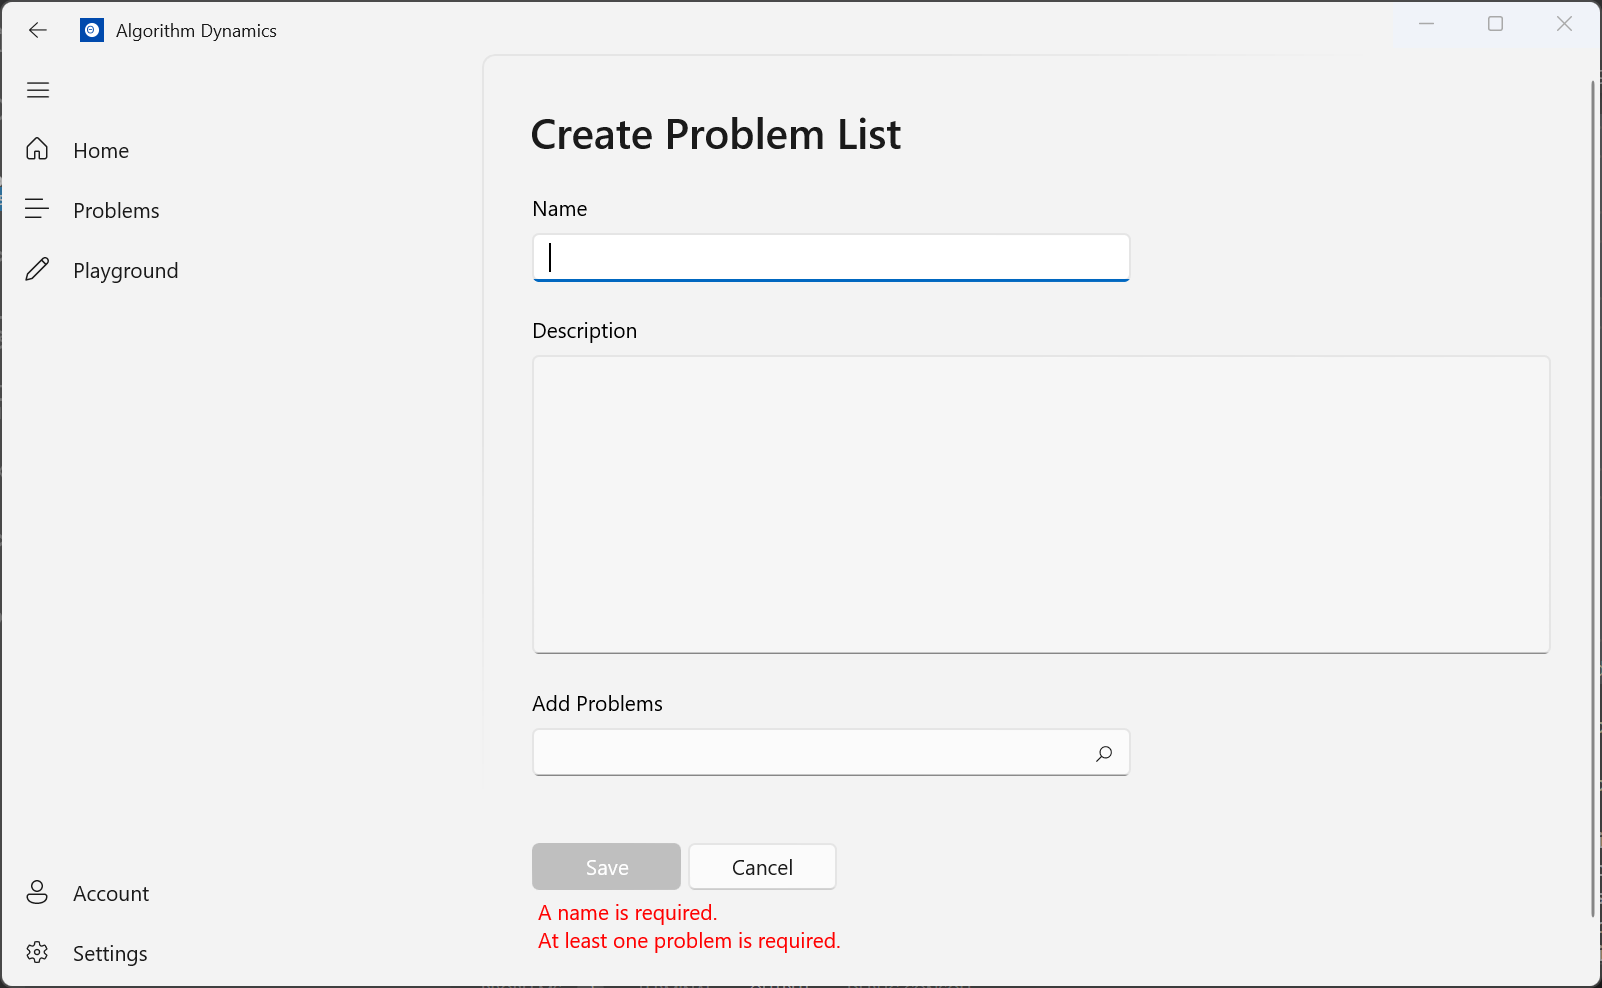
\includegraphics[width=\textwidth, height=\textheight, keepaspectratio]{CreateNewProblemListPage-Testing-Empty}

Invalid input: Pass

Invalid input gets filtered by the controls automatically.

\subsubsection{AccountPage}

Empty input: Pass

No name or email is input, the save button is disabled and a correct error message is displayed.

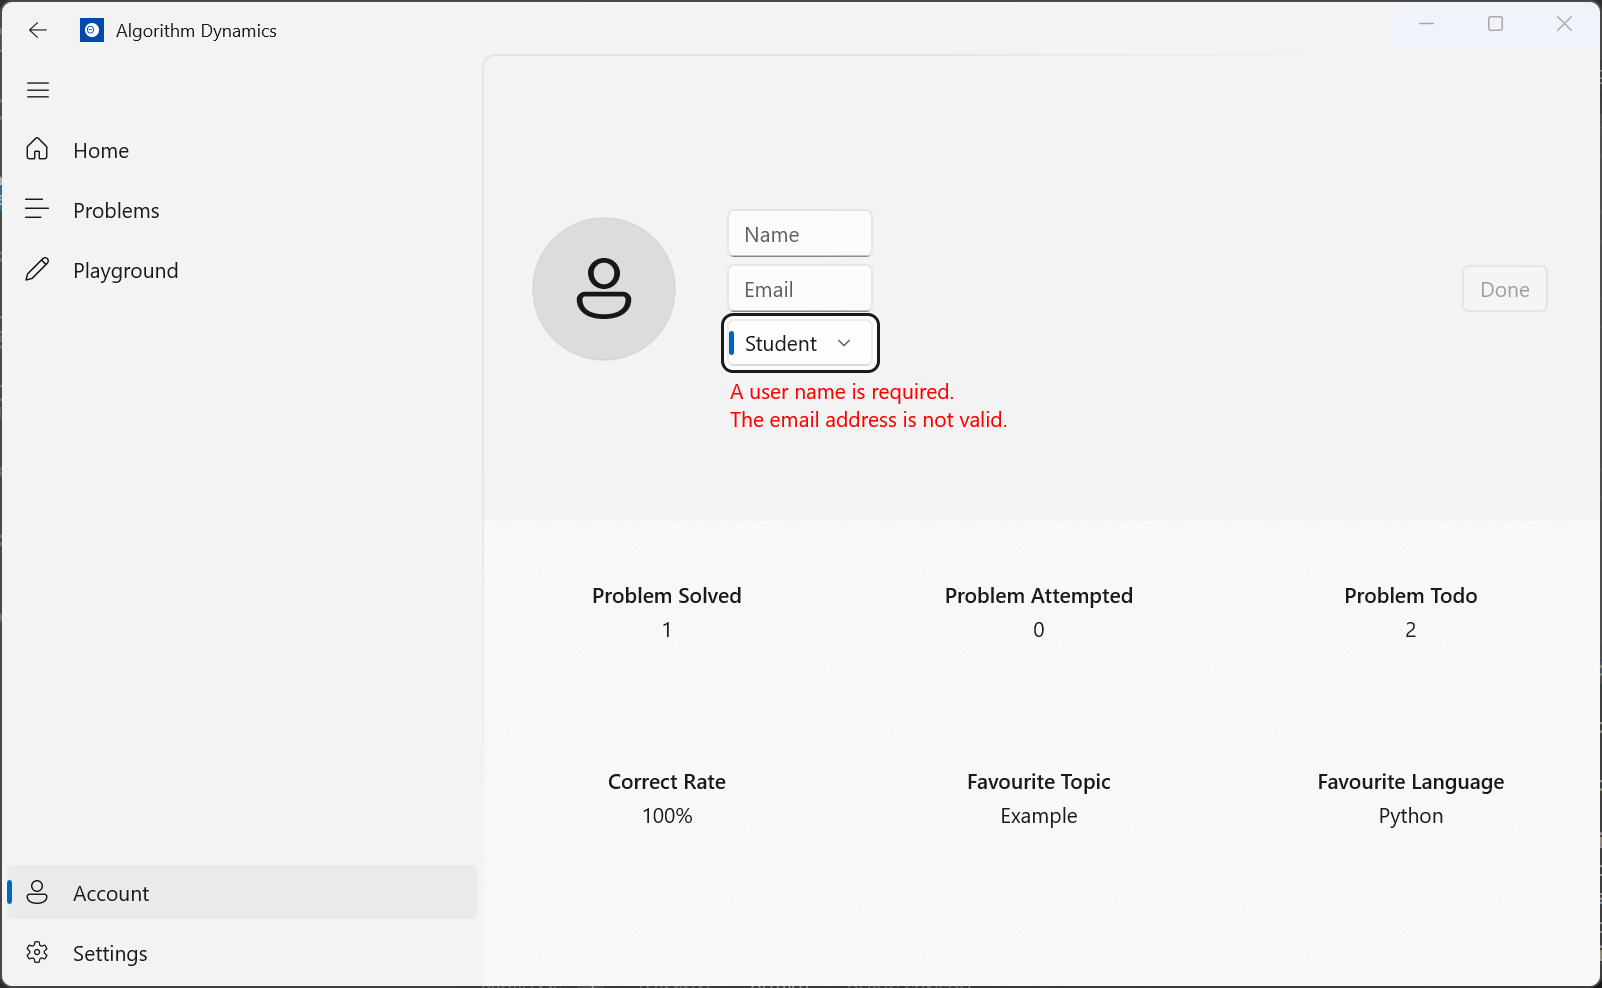
\includegraphics[width=\textwidth, height=\textheight, keepaspectratio]{AccountPage-Testing-Empty}

Invalid input: Pass

Invalid input gets filtered by the controls automatically.

\subsubsection{SettingsPage}

Invalid input: Pass

Invalid input gets filtered by the controls automatically.

Empty input: Pass

A default settings file is generated automatically.

\subsection{Review of the alpha testing}

I am excited to see that all tests passed in the alpha testing. This is mainly because I conduct testing throughout the development stage so all bugs are fixed during the development. There are no usability issues or validation issues. I will conduct a beta test with my stakeholders and gather feedback from them.

\section{Beta testing and review from stakeholders}

\subsection{Beta testing feedback from Mr Grimwood}

Mr Grimwood likes the welcome page on the first launch for registration, and all fields are nicely validated with useful error messages. However, he thinks that there can be more animation and introduction on the welcome page, explaining the purpose of the software. He also thinks after the first login, there can be some teaching tips, about what different pages do and how to navigate around. Mr Grimwood finds the homepage especially useful for him to navigate to different pages easily through Quick Access.

Mr Grimwood points out he can input descriptions for problem lists, but it is not displayed in the app. The description of a problem list should show up when a list is selected in the ProblemsPage somehow.

Mr Grimwood finds it very useful to select multiple problems in the ProblemPage and create a problem list from it directly. This lets him create a problem list and share it with his student very easily.

Mr Grimwood also finds that creating a lot of test cases is very daunting. He says it will be great if test cases can be automatically generated somehow. For example, he can provide a correct code solution and some inputs, and outputs can be executed and recorded automatically. But he likes the problem preview on the create page, so he can preview the problem in real-time. He thinks the database is very robust with good validation. He can't create an invalid problem (with no name/no test cases/invalid limits).

Overall, Mr Grimwood thinks the app is functioning very well, with no crashes and proper validation on all inputs. He thinks it is still a shame that the assignment function can not be implemented though he understands the security issue behind it.

\subsection{Beta testing feedback from PCloud}

PCloud thinks the NavigationView is very useful to navigate around the software, but he says it will be even better if it supports keyboard shortcuts so he does not need to leave the keyboard when using the app.

PCloud likes the code editor, he thinks it has very powerful syntax highlighting and a very nice typing experience. But he says it will be very nice if the code editor can load faster since currently it usually takes around 1 second to load the editor.

PCloud thinks the import/export function is very useful. He can get started quickly by importing a problem list quickly without creating every problem himself. He is particularly satisfied with the performance of the import module. It takes no time to import hundreds of problems and every problem is validated along the way making this process especially useful.

PCloud also enjoys the fuzzy search function in the ProblemsPage, he says this function makes searching in a large problem database easily. He thinks generally the search function works very well, allowing to add of different constraints makes finding the exact problem very easy. He says it will be better if multiple tags can be selected and searched at the same time.

PCloud likes the RunCode function, which allows him to check his code against the example test cases before formal submission. And he likes the progress bar as well which allows him to know the judging progress.

PCloud thinks overall the app has very good performance, and he encounters no crashes while using it. The app takes up very little memory comparing other similar products and it judges the submissions a lot faster than other similar products. PCloud thinks the app runs without an Internet connection makes it especially attractive to him, he finds he can trust the app not selling his data and his privacy is protected.

\subsection{Beta testing feedback from Timofei}

Timofei likes to be able to change the colour theme of the software, the modern design and the dark mode is appealing to him. He thinks the fullscreen button in the CodingPage is very helpful, which creates an immersive working environment and remove all distractions.

Timofei finds the PlaygroundPage page very useful for him to run any short pieces of code without launching a huge IDE. He thinks it can be more useful if the programming language select box can remember his last option instead of resetting to the first language every time.

Timofei finds the statistics in the AccountPage very interesting, after a day of hard work, looking at the stats increases is very satisfying. He thinks there still can be more stats data items shown to make it more inspiring. For example, a coding heat map representing the coding frequency every day.

Timofei thinks the submission grid is very useful for revision, he can see how he got things right or wrong in the past and revise from the mistakes. It will be better if it can be sorted by time or programming language. And if there can be documentation on how to add custom programming languages to the app will be very helpful.

Overall Timofei thinks the app is professional and user friendly. Many features allow him to learn and revise more effectively. He says he will never get tired of learning and practising algorithms and coding in this way.

\subsection{Reviews of the feedback}

My stakeholders generally give very positive feedback about this project. From their feedback, the app seems to meet most of its success criteria. It is very encouraging to see that none of them encounters any crashing or validation errors. The stakeholders also provide a lot of ideas about further improvements that can be done, which I will address in the future.

\section{Success criteria}

\subsection{User experience criteria}

\subsubsection{Easy navigate around the software}

The design of the quick access menu in the HomePage enables one-click access to all core functionalities. The recommendations on the HomePage also allows the user to get into working faster.

The design of the navigation panel on the left enables the user to navigate through different pages at any time. The panel can also expand or collapse so the user can get focused when they are working. This criterion is fully met.

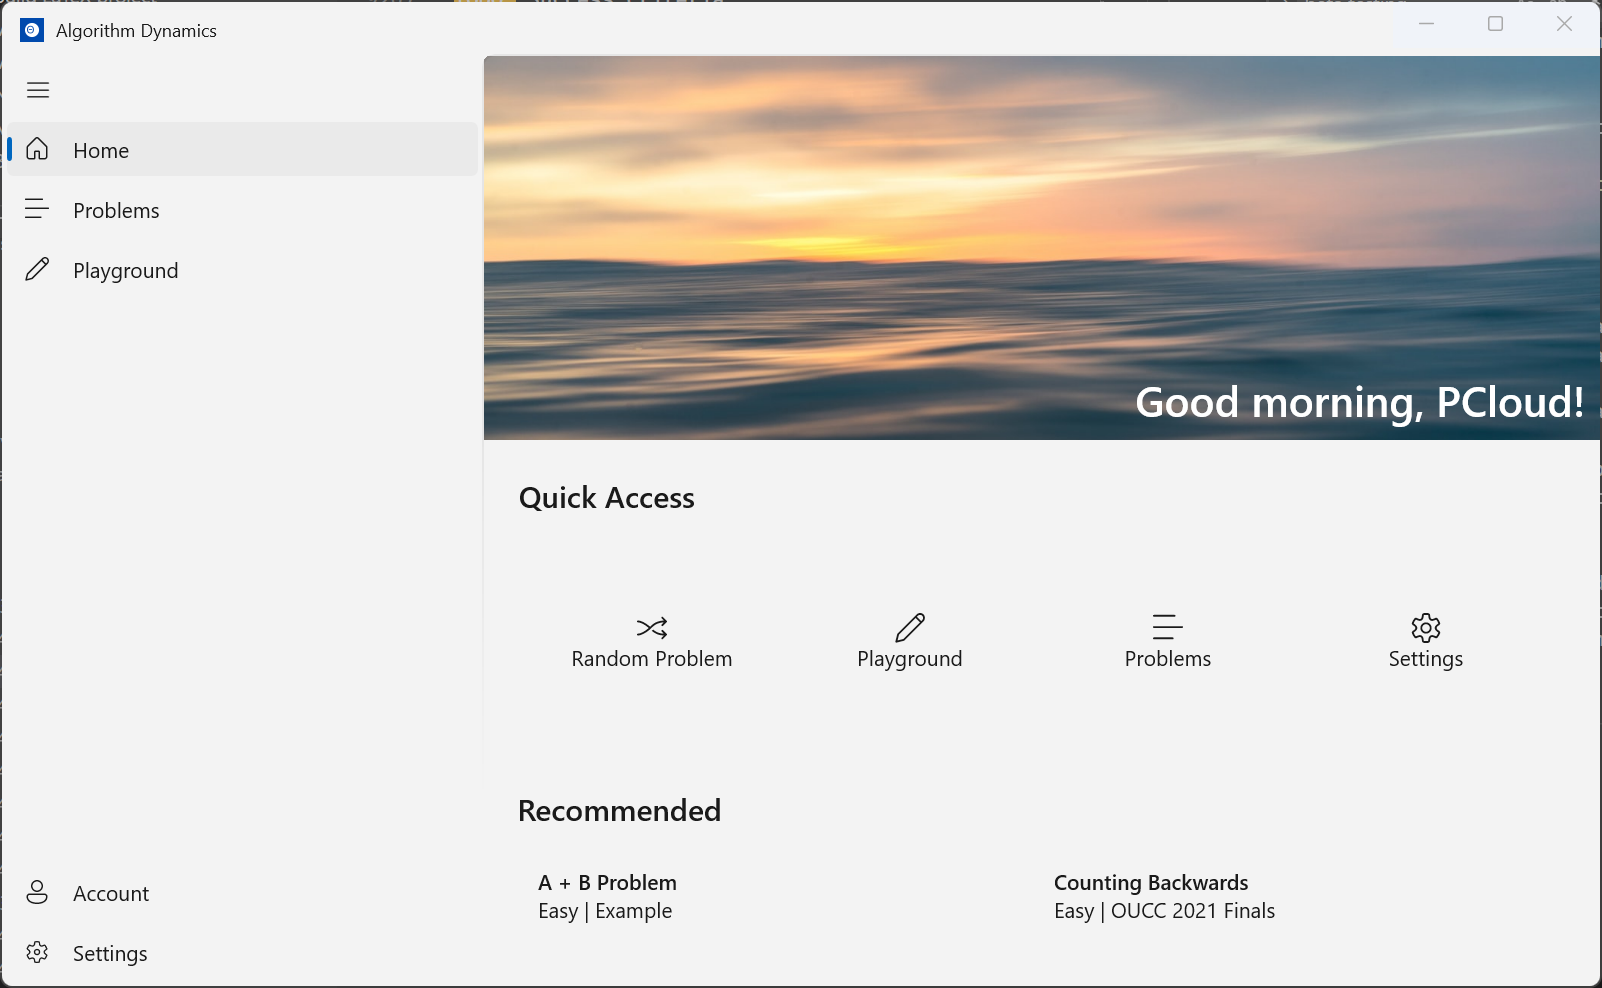
\includegraphics[width=\textwidth, height=\textheight, keepaspectratio]{HomePage-Final}

\subsubsection{Easy to find data in the database}

An advanced search bar is provided for the user to search through the database easily. The user can search based on the difficulty, the tag, the status and the list of the problem. The search box also supports fuzzy search so the user does not need to remember the exact name of the problem. This criterion is fully met.

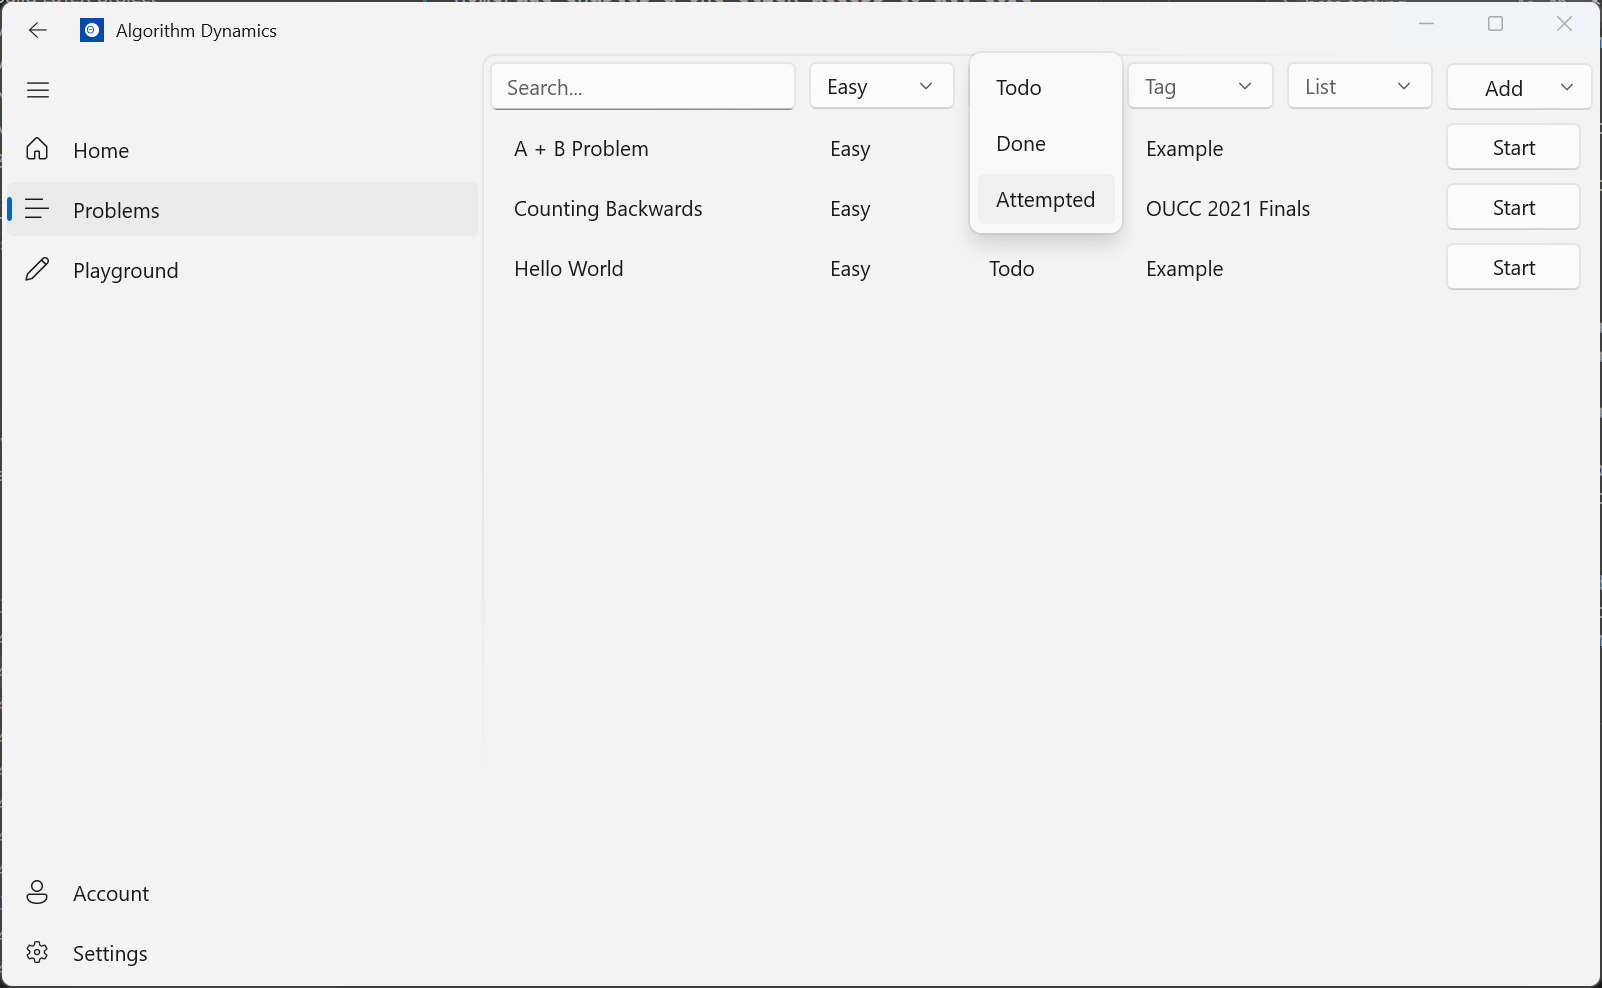
\includegraphics[width=\textwidth, height=\textheight, keepaspectratio]{ProblemsPage-Final}

\subsubsection{Easy to create new problems}

A CreateNewProblemPage is provided for the user to create a new problem easily. It provides text and number input boxes for the user to input problem details. Default values are provided for the problem properties. A template is provided for the problem description. A markdown preview panel is provided for preview. This criterion is fully met.

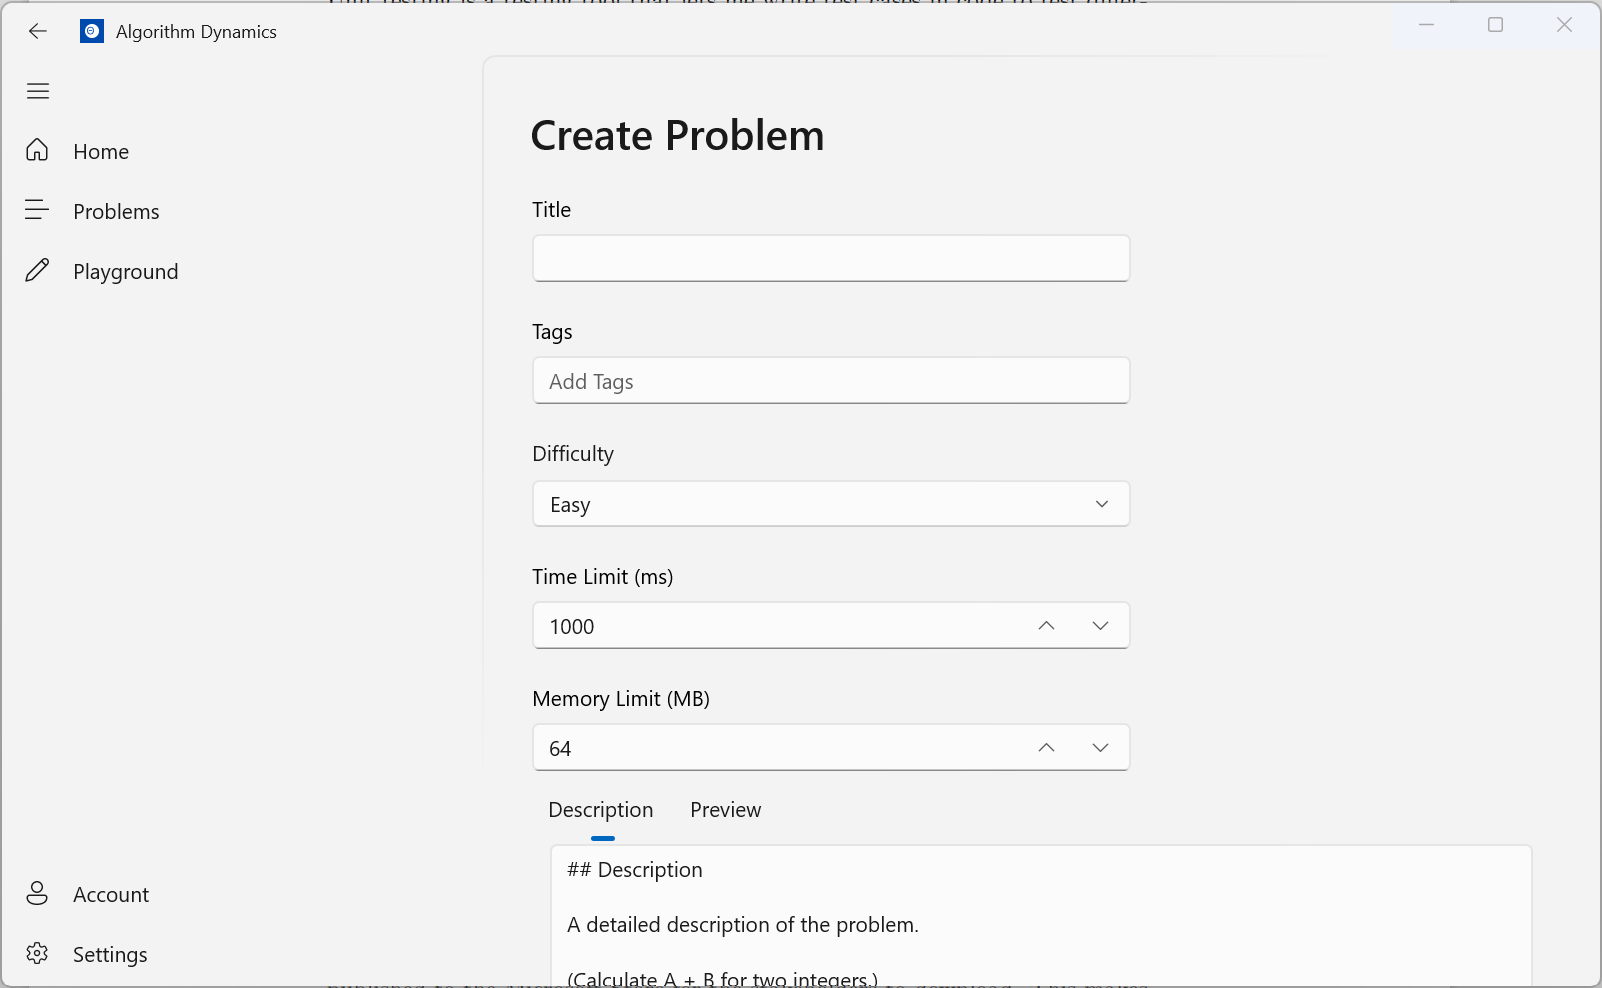
\includegraphics[width=\textwidth, height=\textheight, keepaspectratio]
{CreateNewProblemPage-Final}

\subsubsection{Easy to create new problem lists}

A CreateNewProblemListPage is provided for the user to create a new problem list easily. It provides text input boxes for the user to input details. A search box is provided for the user to search and add new problems easily. This criterion is fully met.

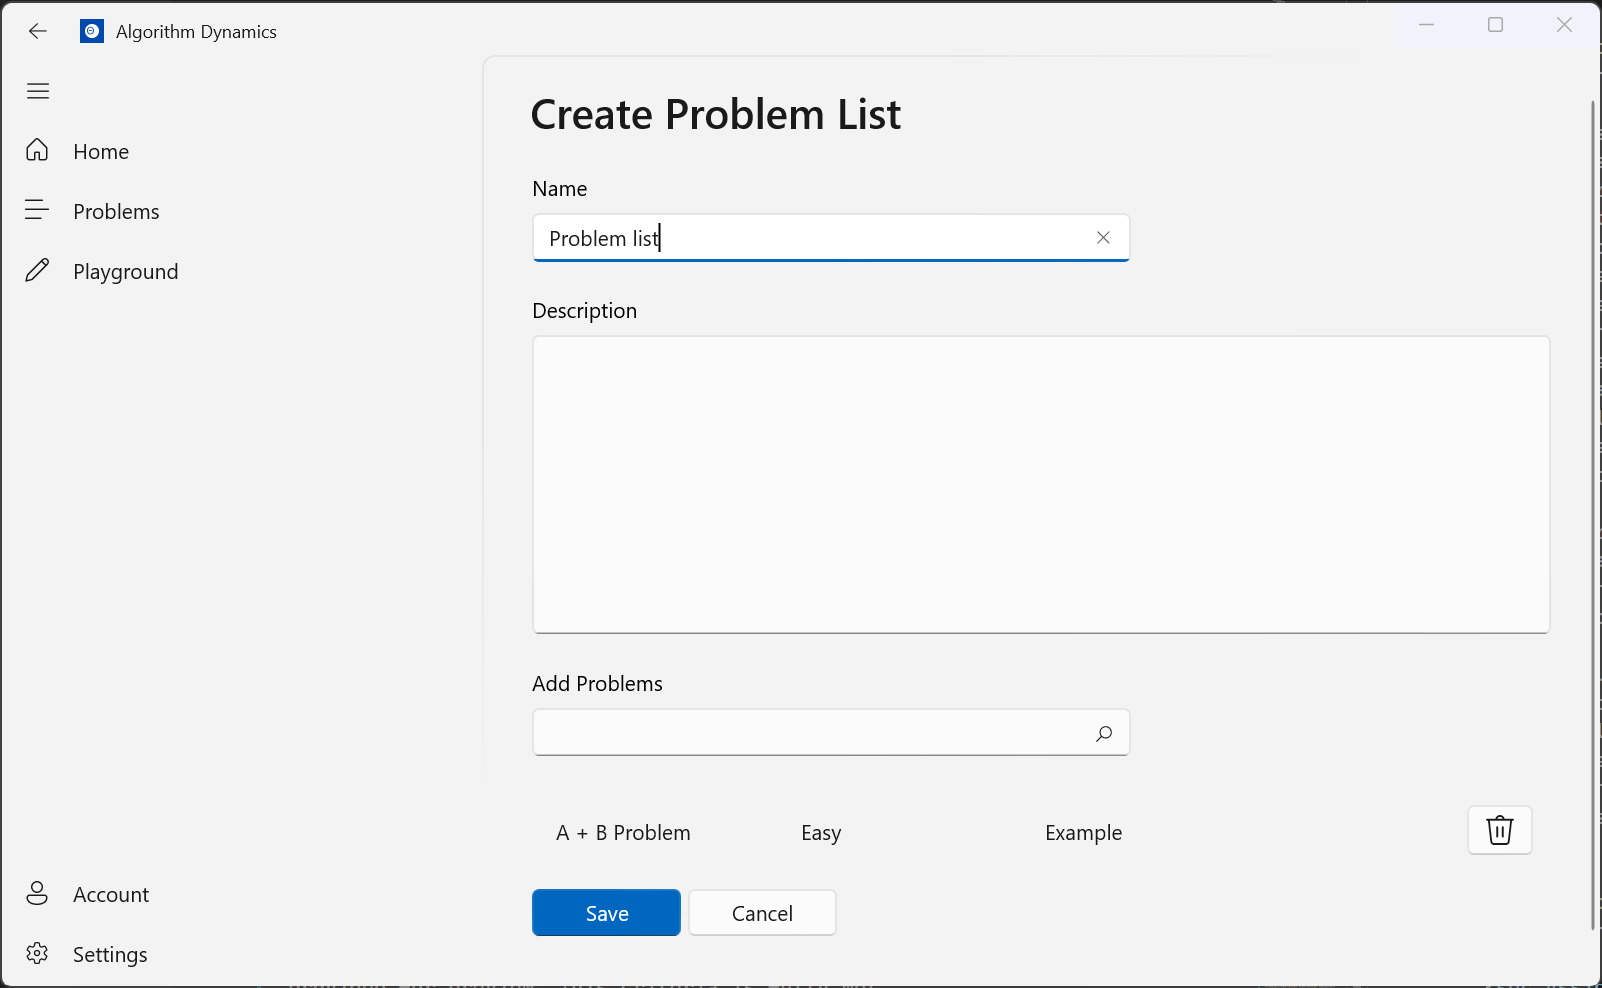
\includegraphics[width=\textwidth, height=\textheight, keepaspectratio]{CreateNewProblemListPage-Final}

\subsubsection{Assignment functionality}

Due to a security flaw in design reported by one of my stakeholders during the development stage, the assignment functionality is cancelled. Allowing any code submission from students to be executed on the teacher's computer without any permission control is very dangerous, potentially causing the teacher's computer to be hacked or data to be leaked. However, there is no easy way of implementing permission control and therefore this functionality is cancelled and this criterion is not met.

\subsubsection{Microsoft Teams integration}

Due to the assignment functionality being cancelled, there is not much point in implementing the Microsoft Teams integration alone. Also because I don't have the permission to call and debug education API as explained in the development stage, the Microsoft Teams integration is cancelled. This criterion is not met.

\subsubsection{Playground functionality}

A PlaygroundPage is provided for the user to run any code in any programming language with customer input. The user can also set the time limit or the memory limit to prevent the code from running forever. This criterion is fully met.

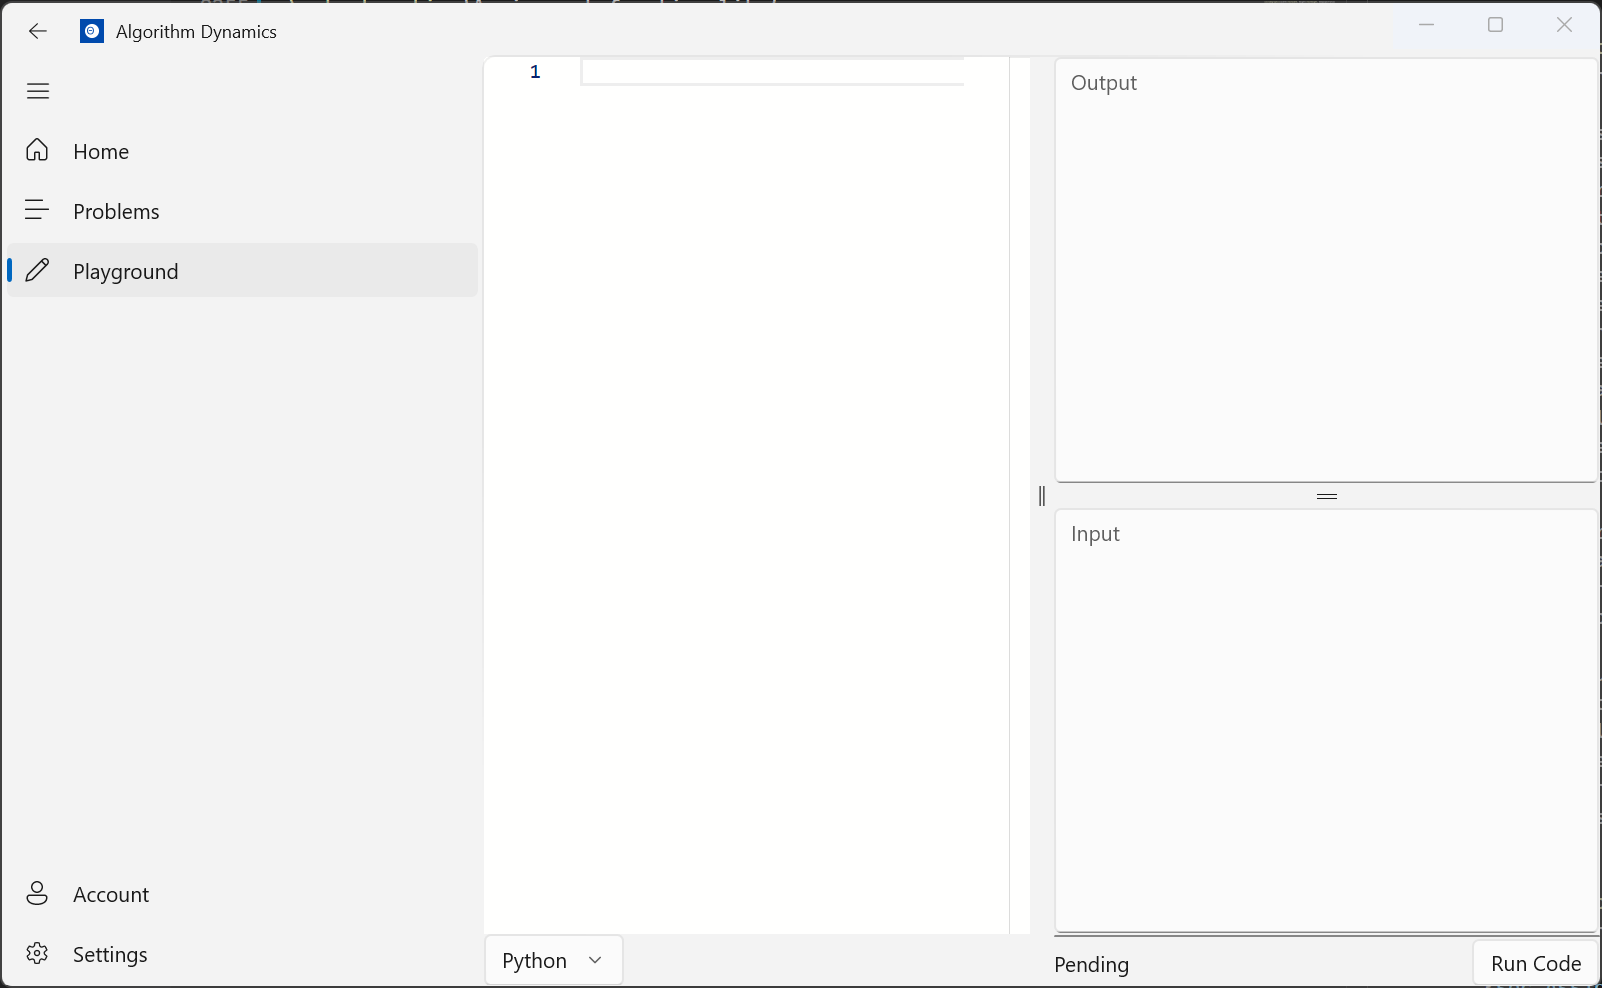
\includegraphics[width=\textwidth, height=\textheight, keepaspectratio]{PlaygroundPage-Final}

\subsubsection{Custom settings options}

A SettingsPage is provided for the user to adjust settings such as light/dark mode, playground limits, programming language settings and clear database. The setting persists between sessions initialized automatically on the first launch and deleted automatically when the app is uninstalled. This criterion is fully met.

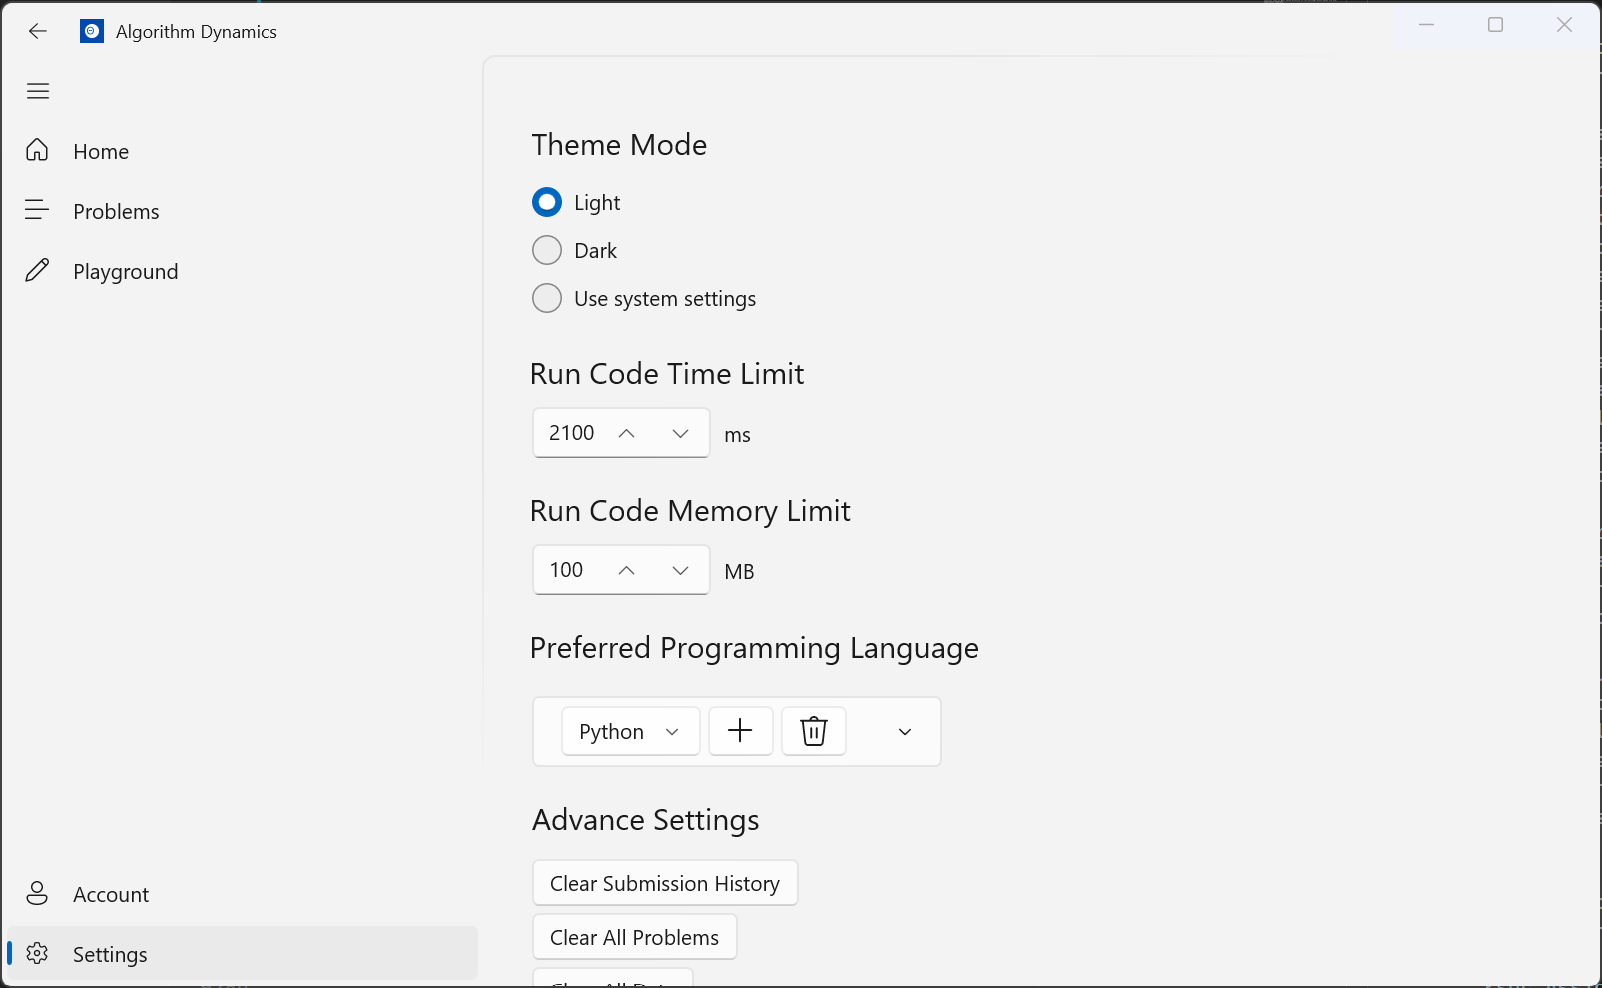
\includegraphics[width=\textwidth, height=\textheight, keepaspectratio]{SettingsPage-Final}

\subsubsection{Account settings}

An AccountPage is provided for the user to edit account settings such as user name and email. But due to the AssignmentPage being cancelled, this part of the information is not utilized. It also provides statistical data related to the account, which is very useful based on the stakeholder's feedback. This criterion is fully met.

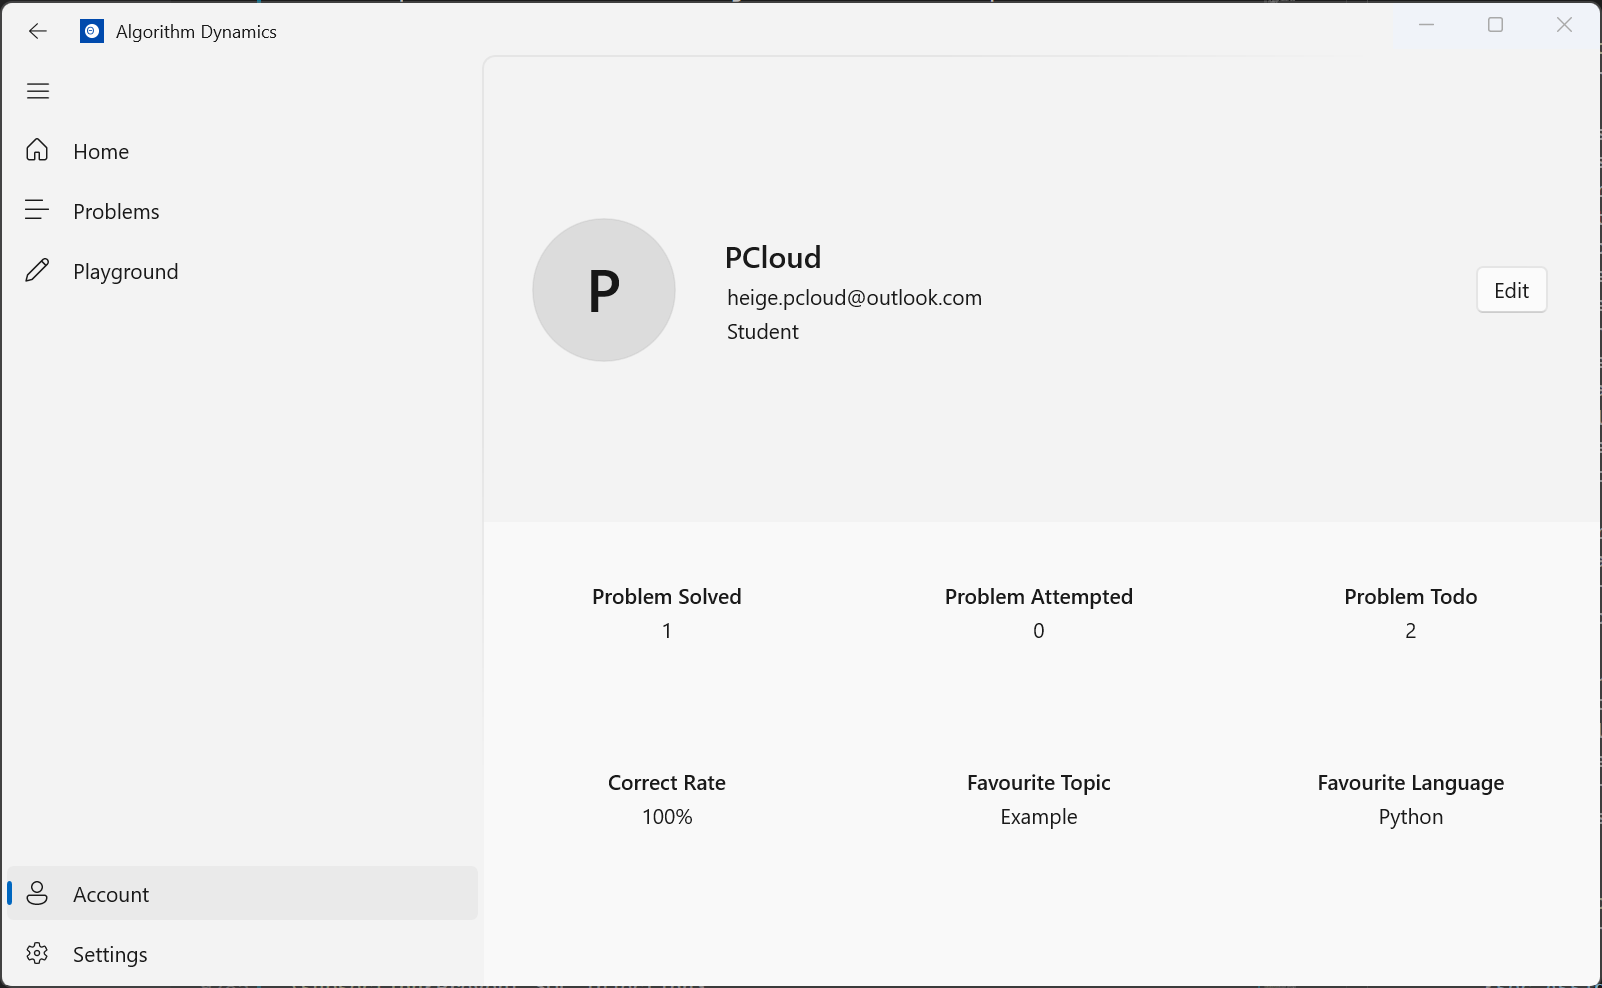
\includegraphics[width=\textwidth, height=\textheight, keepaspectratio]{AccountPage-Final}

\subsection{Technical criterias}

\subsubsection{Local Database}

All unit tests on the DataAccess class passes, which means the database is working as expected. In the black box test and the integration test, no issue with the local database is discovered. It is created successfully when the app is run the first time. This criterion is fully met.

\subsubsection{Prevent SQL injection}

The entire DataAccess class is using the parameterized solution, so all variable fields are treated as variables and no string concatenation is used. It is impossible to inject SQL into the database. This criterion is fully met.

\subsubsection{Data validation}

As tested in the alpha testing stage and the beta testing stage, all fields are validated in the user interface and a useful error message is provided to the user. This criterion is fully met.

\subsubsection{Code Editor}

The code editor supports line number, syntax highlighting, code folding, code completion, and code navigation. This criterion is fully met.

\subsubsection{API calls}

This criterion is not met. Since the Teams integration is forced to be cancelled.

\subsubsection{Meaningful variale name}

All variables use meaningful names. This criterion is fully met. Please refer to the source code for details.

\subsubsection{Comments}

All important functions and codes are associated with comments explaining their purpose. This criterion is fully met. Please refer to the source code for details.

\subsubsection{Object Oriented Design}

All pages, data models are designed using OOP. This criterion is fully met.

\subsubsection{Modular design}

The entire app is split into 3 small projects. Algorithm Dynamics contains all code for user interface logic, Algorithm Dynamics.Core contains all the code for the database and the judger, Algorithm Dynamics.Test contains all the unit tests for core functionalities. I use OOP design throughout the development, each page, window, the data model is all abstracted into a class. Thus I can conclude that the code is modular and easy to maintain. This criterion is fully met.

\subsubsection{Continuous integration and continuous delivery}

I have set up a CI/CD pipeline from the beginning, each time when I modify the source code, the CI/CD tasks are run automatically to build and test the code. When I release a new version of the app, a release is automatically created and sent to the Microsoft Store. This criterion is fully met.

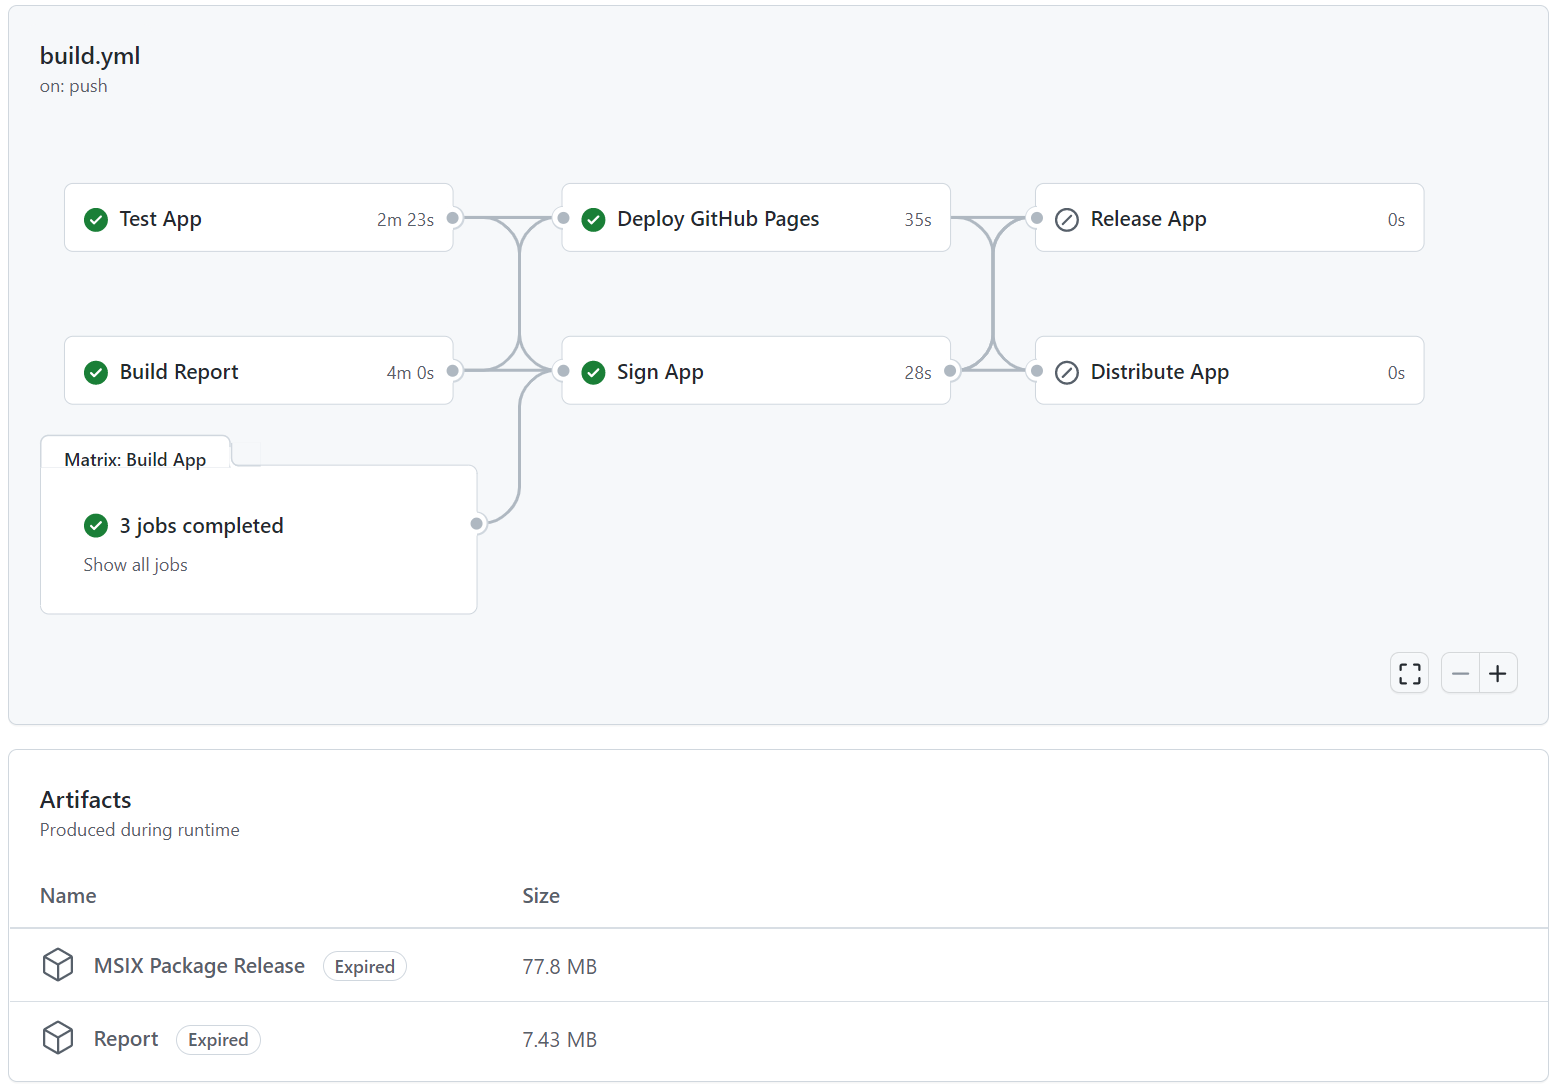
\includegraphics[width=\textwidth, height=\textheight, keepaspectratio]{CICD}

\subsubsection{Unit test for core functions}

All unit tests for the core functions are passed with a code coverage above 88\%. This makes sure the core library is bug-free and therefore this criterion is fully met.

\section{Limitations, further maintenance and developement}

\subsection{Cross platform}

The current app only runs on Windows by design, so Linux or macOS users will not be able to use it. It is okay for all my stakeholders, but in real life, there are a lot of users who do not work on a Windows device. It will be really useful for the app to support multiple platforms, so it can reach more users and help more students and teachers.

The current code base is heavily dependent on the dotnet runtime and the WinUI 3 library and there is no easy way to make it cross-platform in one click.

One possible solution is the new .NET MAUI framework\cite{microsoft:docs:what-is-maui}, which is currently in its beta development phase. It also depends on the dotnet runtime, which means I can reuse most of my existing codebase. But since it is still in the beta testing phase, and there are a lot of bugs and unsupported features, currently it is not possible to migrate to this framework.

The other solution is to completely rewrite the app using web technologies, which can run on any browser, and therefore any device. I can also use technologies like ElectronJS\cite{electron} to pack the webpages into a desktop app for offline use. I personally do not agree with this approach, since I need to rewrite the entire codebase, and the result will probably have much worse performance and more limitations.

In conclusion, it is a very difficult challenge to support multiple platforms, and it will be a long term task.

\subsection{A more flexible Judger}

The current Judger is not very smart, it only takes in pre-generated test cases and makes direct comparisons. There are a lot of ways to make the Judger smarter and provide more useful outputs.

One simple improvement is to allow the user to set up different scores for each test case. For example, passing a simple and small test case is awarded 1 point, while passing a complex test case is awarded 5 points. In the end, instead of passing or not, a numerical score is presented. This allows the teacher to get more information about students.

Another improvement is to support the custom special judge. In some cases, there might be more than one possible solution. For example, when there are multiple answers and the order of them does not matter. Instead of simply comparing the outputs, the user can write a custom special judger to determine whether the output is correct.

These tasks are fairly simple to implement since the underlying architecture is designed to be modular and flexible and easy to maintain.

\subsection{Assignment function}

As I mentioned in the development stage, there is no easy way on the Windows operating system to run external code safely. One possible approach is to send the code to a remote server, and then run the code in a virtual machine or a docker container so it cannot cause any damage, and then send the result back. This requires extra servers and exchanging data, which is a giant task. There might also involve some legal issues since a server storing student submission code may need to comply with the GDPR. An alternative is to allow the teacher to host the judger on a local server, but this also needs extra work and will not be easy to set up. Overall, there is no simple alternative solution to this problem and I will keep researching to find a proper solution before implementing it.

\subsection{Assignment integration}

I find I can't integrate my app with the Microsoft Education API since it requires an account from an education organization, which I do not have and probably will never have. It might be possible to integrate the app with other education apps such as Slack or Google Classroom. More in-depth research needs to be done to determine if this is possible. This task also depends on the assignment function, so it probably will not be done shortly.

\subsection{A better code editor}

The current code editor is based on the web view and the Monaco Editor. Compared to a native editor, it is fairly slow. Some upstream bugs of the web view component also cause many inconvenient issues in the implementation. A native code editor, supporting line number, syntax highlighting, find and replace is desirable.

Implementing a code editor from scratch is very difficult. There is no similar project written in C\#, I can implement it as a standalone library so other people can benefit from it as well. This will be a long term task.

\subsection{Unit test for UI}

I added unit tests for Algorithm Dynamics.Core throughout its development. And I have seen how useful unit test is to eliminate bugs during the development stage. It will be very helpful if I can add unit tests for the UI code as well.

One possible way is to refactor the UI code into the MVVM\cite{microsoft:docs:mvvm-introduction} pattern, which abstracts a view model out of the UI and decouples the UI logic with its markup using data binding\cite{microsoft:docs:data-binding-and-mvvm}. I have heavily used data binding throughout the development and the refactor will take a lot of work but it should be pretty straightforward. After the abstraction of the view model, I can write test cases in the Algorithm Dynamics.Test project to test the behaviour of the view models just like testing the DataAccess and Judger class. However, currently, it is not possible to connect an MSTest project to a WinUI 3 project due to some upstream limitations\cite{github:microsoft-ui-xaml:6258}. But I can start refactoring, which also makes the code easier to be maintained, and start writing unit tests once this feature is supported.

\subsection{Stakeholder suggestions}

On top of everything mentioned above, my stakeholders have given me a lot of suggestions that I can work on as well. This includes:

\begin{itemize}
  \item Better beginner's guide with animation and teaching tips.
  \item Utilize the problem list descriptions.
  \item More keyboard shortcuts.
  \item Faster code editor.
  \item Multiple tags in the search box.
  \item More graphical statistics data.
  \item Better submission grid with sorting and searching.
\end{itemize}

I will try to make some initial designs of these improvements and fully discuss them with my stakeholders. After which these can be implemented in the future easily.

\end{document}